% Seminar 2: Distribuții Clasice --- Normal și Student-t

\documentclass[9pt, aspectratio=169, t]{beamer}
%=============================================================================
% PREAMBUL COMUN - Statistica Piețelor Financiare
% Prezentări academice de calitate Harvard
% Program de licență, Academia de Studii Economice din București
%
% Utilizare: \documentclass[9pt, aspectratio=169, t]{beamer}
%            %=============================================================================
% PREAMBUL COMUN - Statistica Piețelor Financiare
% Prezentări academice de calitate Harvard
% Program de licență, Academia de Studii Economice din București
%
% Utilizare: \documentclass[9pt, aspectratio=169, t]{beamer}
%            %=============================================================================
% PREAMBUL COMUN - Statistica Piețelor Financiare
% Prezentări academice de calitate Harvard
% Program de licență, Academia de Studii Economice din București
%
% Utilizare: \documentclass[9pt, aspectratio=169, t]{beamer}
%            \input{preamble}
%            \subtitle{Seminar X: Titlul Seminarului}
%            \begin{document} ...
%=============================================================================

% Asigură încadrarea conținutului pe diapozitive
\setbeamersize{text margin left=8mm, text margin right=8mm}

%=============================================================================
% CONFIGURARE TEMĂ ȘI STIL
%=============================================================================
\usetheme{default}

% Paletă de Culori
\definecolor{MainBlue}{RGB}{26, 58, 110}
\definecolor{AccentBlue}{RGB}{26, 58, 110}
\definecolor{IDAred}{RGB}{205, 0, 0}
\definecolor{DarkGray}{RGB}{51, 51, 51}
\definecolor{MediumGray}{RGB}{128, 128, 128}
\definecolor{LightGray}{RGB}{248, 248, 248}
\definecolor{VeryLightGray}{RGB}{235, 235, 235}
\definecolor{KeynoteGray}{RGB}{218, 218, 218}
\definecolor{SectionGray}{RGB}{120, 120, 120}
\definecolor{FooterGray}{RGB}{100, 100, 100}
\definecolor{Crimson}{RGB}{220, 53, 69}
\definecolor{Forest}{RGB}{46, 125, 50}
\definecolor{Amber}{RGB}{181, 133, 63}
\definecolor{Orange}{RGB}{230, 126, 34}
\definecolor{Purple}{RGB}{142, 68, 173}

% Fundal gradient (gradient Keynote exact 315°: alb la RGB 218,218,218)
\setbeamertemplate{background}{%
    \begin{tikzpicture}[remember picture, overlay]
        \shade[shading=axis, shading angle=315,
        top color=white, bottom color=KeynoteGray]
        (current page.south west) rectangle (current page.north east);
    \end{tikzpicture}%
}
% Culoare solidă de rezervă pentru compatibilitate
\setbeamercolor{background canvas}{bg=}

\setbeamercolor{palette primary}{bg=MainBlue, fg=white}
\setbeamercolor{palette secondary}{bg=MainBlue!85, fg=white}
\setbeamercolor{palette tertiary}{bg=MainBlue!70, fg=white}
\setbeamercolor{structure}{fg=MainBlue}
\setbeamercolor{title}{fg=IDAred}
\setbeamercolor{frametitle}{fg=IDAred, bg=}
\setbeamercolor{block title}{bg=MainBlue, fg=white}
\setbeamercolor{block body}{bg=VeryLightGray, fg=DarkGray}
\setbeamercolor{block title alerted}{bg=Crimson, fg=white}
\setbeamercolor{block body alerted}{bg=Crimson!8, fg=DarkGray}
\setbeamercolor{block title example}{bg=Forest, fg=white}
\setbeamercolor{block body example}{bg=Forest!8, fg=DarkGray}
\setbeamercolor{item}{fg=MainBlue}

% Font institute mai mic pentru a evita overfull hbox pe pagina de titlu
\setbeamerfont{institute}{size=\footnotesize}

% Culori subsol
\setbeamercolor{author in head/foot}{fg=FooterGray, bg=}
\setbeamercolor{title in head/foot}{fg=FooterGray, bg=}
\setbeamercolor{date in head/foot}{fg=FooterGray, bg=}
\setbeamercolor{section in head/foot}{fg=FooterGray, bg=}
\setbeamercolor{subsection in head/foot}{fg=FooterGray, bg=}

% Stiluri marcatori
\setbeamertemplate{itemize item}{\color{MainBlue}$\boxdot$}
\setbeamertemplate{itemize subitem}{\color{MainBlue}$\blacktriangleright$}
\setbeamertemplate{itemize subsubitem}{\color{MainBlue}\tiny$\bullet$}
\setbeamertemplate{itemize/enumerate body begin}{\normalsize}
\setbeamertemplate{itemize/enumerate subbody begin}{\normalsize}

% Stiluri cuprins (bullets în loc de numere)
\setbeamertemplate{section in toc}{%
    \leavevmode\leftskip=1.5em%
    \llap{\color{MainBlue}$\boxdot$\kern0.5em}%
    \inserttocsection\par%
}

% Spațiere compactă
\setlength{\leftmargini}{10pt}
\setlength{\leftmarginii}{10pt}
\makeatletter
\def\@listi{\leftmargin\leftmargini \topsep 0pt \parsep 0pt \itemsep 0pt}
\def\@listii{\leftmargin\leftmarginii \topsep 0pt \parsep 0pt \itemsep 0pt}
\makeatother

\setbeamertemplate{navigation symbols}{}

%=============================================================================
% ANTET PERSONALIZAT
%=============================================================================
\setbeamertemplate{headline}{%
    \vskip10pt%
    \hbox to \paperwidth{%
        \hskip0.5cm%
        {\small\color{FooterGray}\renewcommand{\hyperlink}[2]{##2}\insertsectionhead}%
        \hfill%
        \textcolor{FooterGray}{\small\insertframenumber}%
        \hskip0.5cm%
    }%
    \vskip4pt%
    {\color{FooterGray}\hrule height 0.4pt}%
}

%=============================================================================
% SUBSOL PERSONALIZAT
%=============================================================================
\usepackage{fontawesome5}

\setbeamertemplate{footline}{%
    {\color{FooterGray}\hrule height 0.4pt}%
    \vskip4pt%
    \hbox to \paperwidth{%
        \hskip0.5cm%
        \textcolor{FooterGray}{\small Statistica Piețelor Financiare}%
        \hfill%
        \raisebox{-0.1em}{%
            \begin{tikzpicture}[x=0.08em, y=0.08em, line width=0.4pt]
                \draw[FooterGray] (0,3) -- (1,4) -- (2,3.5) -- (3,5) -- (4,4) -- (5,6) -- (6,5.5) -- (7,4) -- (8,5) -- (9,7) -- (10,6) -- (11,5) -- (12,6.5) -- (13,8) -- (14,7) -- (15,6) -- (16,7.5) -- (17,9) -- (18,8) -- (19,7) -- (20,8.5) -- (21,10) -- (22,9) -- (23,8) -- (24,9.5);
            \end{tikzpicture}%
        }%
        \hskip0.5cm%
    }%
    \vskip6pt%
}

%=============================================================================
% PACHETE
%=============================================================================
\usepackage[utf8]{inputenc}
\usepackage[T1]{fontenc}
\usepackage{amsmath, amssymb, amsthm}
\usepackage{mathtools}
\usepackage{bm}
\usepackage{tikz}
\usetikzlibrary{arrows.meta, positioning, shapes, calc, decorations.pathreplacing, shadings}
\usepackage{booktabs}
\usepackage{multirow}
\usepackage{array}
\usepackage{graphicx}
\usepackage{hyperref}
\usepackage{colortbl}
\usepackage{listings}
\lstset{basicstyle=\ttfamily\small, breaklines=true, frame=single, backgroundcolor=\color{VeryLightGray}}
\hypersetup{colorlinks=true, linkcolor=MainBlue, urlcolor=MainBlue}
\graphicspath{{../../logos/}{../../charts/}{../../photos/}}
\hfuzz=2pt
\vfuzz=2pt

%=============================================================================
% COMANDA QUANTLET
%=============================================================================
\newcommand{\quantlet}[2]{%
    \hfill\href{#2}{%
        \raisebox{-0.15em}{
\includegraphics[height=0.7em]{ql_logo.png}}%
        \textcolor{MainBlue}{\tiny\ #1}%
    }%
}

%=============================================================================
% PAGINĂ TITLU PERSONALIZATĂ
%=============================================================================
\defbeamertemplate*{title page}{hybrid}[1][]
{
    \vspace{0.2cm}
    \begin{center}
        \href{https://www.ase.ro}{
\includegraphics[height=1.0cm]{ase_logo.png}}\hspace{0.25cm}%
        \href{https://theida.net}{
\includegraphics[height=1.0cm]{ida_logo.png}}\hspace{0.25cm}%
        \href{https://blockchain-research-center.com}{
\includegraphics[height=1.0cm]{brc_logo.png}}\hspace{0.25cm}%
        \href{https://www.ai4efin.ase.ro}{
\includegraphics[height=1.0cm]{ai4efin_logo.png}}\hspace{0.25cm}%
        \href{https://ipe.ro/new}{
\includegraphics[height=1.0cm]{acad_logo.png}}\hspace{0.25cm}%
        \href{https://www.digital-finance-msca.com}{
\includegraphics[height=1.0cm]{msca_logo.png}}%
    \end{center}

    \vspace{0.6cm}

    \begin{center}
        \begin{minipage}{0.1\textwidth}
            \centering
            \href{https://quantlet.com}{
\includegraphics[height=1.1cm]{ql_logo.png}}
        \end{minipage}%
        \begin{minipage}{0.78\textwidth}
            \centering
            {\LARGE\bfseries\usebeamercolor[fg]{title}\inserttitle}

            \vspace{0.3cm}

            {\usebeamerfont{subtitle}\usebeamercolor[fg]{title}\insertsubtitle}
        \end{minipage}%
        \begin{minipage}{0.1\textwidth}
            \centering
            \href{https://quantinar.com}{
\includegraphics[height=1.1cm]{qr_logo.png}}
        \end{minipage}
    \end{center}

    \vspace{0.6cm}

    \hspace{0.5cm}{\usebeamerfont{author}\insertauthor}

    \vspace{0.3cm}

    \hspace{0.5cm}\begin{minipage}[t]{0.9\textwidth}
        \raggedright\small\insertinstitute
    \end{minipage}
}

%=============================================================================
% MEDII PENTRU TEOREME
%=============================================================================
\theoremstyle{definition}
\setbeamertemplate{theorems}[numbered]
\newtheorem{defn}{Definiție}
\newtheorem{thm}{Teoremă}
\newtheorem{prop}{Propoziție}
\newtheorem{rmk}{Observație}

%=============================================================================
% CENTRED MINIPAGE
%=============================================================================
\newenvironment{cminipage}[1]{%
    \par\noindent\hfill\begin{minipage}{#1}\ignorespaces
}{%
    \end{minipage}\hfill\null\par
}

%=============================================================================
% COMENZI PERSONALIZATE
%=============================================================================
\newcommand{\E}{\mathbb{E}}
\newcommand{\Var}{\text{Var}}
\newcommand{\Cov}{\text{Cov}}
\newcommand{\Corr}{\text{Corr}}
\newcommand{\R}{\mathbb{R}}
\newcommand{\N}{\mathbb{N}}
\newcommand{\Z}{\mathbb{Z}}
\newcommand{\B}{\mathbf{B}}
\newcommand{\imark}{\textcolor{MainBlue}{\textbullet}}
\newcommand{\RMSE}{\text{RMSE}}
\newcommand{\MAE}{\text{MAE}}
\newcommand{\MAPE}{\text{MAPE}}
\newcommand{\correct}{\textcolor{Forest}{\checkmark}}
\newcommand{\incorrect}{\textcolor{Crimson}{\texttimes}}

%=============================================================================
% INFORMAȚII TITLU
%=============================================================================
\title[Statistica Piețelor Financiare]{Statistica Piețelor Financiare}
\author[D.T. Pele, A. Amza]{\texorpdfstring{\begin{tabular}[t]{@{}l@{}}Daniel Traian PELE \\ Antoaneta Amza\end{tabular}}{Daniel Traian PELE, Antoaneta Amza}}
\institute{Academia de Studii Economice din București\\
IDA Institute Digital Assets\\
Blockchain Research Center\\
AI4EFin Artificial Intelligence for Energy Finance\\
Academia Română, Institutul de Prognoză Economică\\
MSCA Digital Finance}
\date{}

%            \subtitle{Seminar X: Titlul Seminarului}
%            \begin{document} ...
%=============================================================================

% Asigură încadrarea conținutului pe diapozitive
\setbeamersize{text margin left=8mm, text margin right=8mm}

%=============================================================================
% CONFIGURARE TEMĂ ȘI STIL
%=============================================================================
\usetheme{default}

% Paletă de Culori
\definecolor{MainBlue}{RGB}{26, 58, 110}
\definecolor{AccentBlue}{RGB}{26, 58, 110}
\definecolor{IDAred}{RGB}{205, 0, 0}
\definecolor{DarkGray}{RGB}{51, 51, 51}
\definecolor{MediumGray}{RGB}{128, 128, 128}
\definecolor{LightGray}{RGB}{248, 248, 248}
\definecolor{VeryLightGray}{RGB}{235, 235, 235}
\definecolor{KeynoteGray}{RGB}{218, 218, 218}
\definecolor{SectionGray}{RGB}{120, 120, 120}
\definecolor{FooterGray}{RGB}{100, 100, 100}
\definecolor{Crimson}{RGB}{220, 53, 69}
\definecolor{Forest}{RGB}{46, 125, 50}
\definecolor{Amber}{RGB}{181, 133, 63}
\definecolor{Orange}{RGB}{230, 126, 34}
\definecolor{Purple}{RGB}{142, 68, 173}

% Fundal gradient (gradient Keynote exact 315°: alb la RGB 218,218,218)
\setbeamertemplate{background}{%
    \begin{tikzpicture}[remember picture, overlay]
        \shade[shading=axis, shading angle=315,
        top color=white, bottom color=KeynoteGray]
        (current page.south west) rectangle (current page.north east);
    \end{tikzpicture}%
}
% Culoare solidă de rezervă pentru compatibilitate
\setbeamercolor{background canvas}{bg=}

\setbeamercolor{palette primary}{bg=MainBlue, fg=white}
\setbeamercolor{palette secondary}{bg=MainBlue!85, fg=white}
\setbeamercolor{palette tertiary}{bg=MainBlue!70, fg=white}
\setbeamercolor{structure}{fg=MainBlue}
\setbeamercolor{title}{fg=IDAred}
\setbeamercolor{frametitle}{fg=IDAred, bg=}
\setbeamercolor{block title}{bg=MainBlue, fg=white}
\setbeamercolor{block body}{bg=VeryLightGray, fg=DarkGray}
\setbeamercolor{block title alerted}{bg=Crimson, fg=white}
\setbeamercolor{block body alerted}{bg=Crimson!8, fg=DarkGray}
\setbeamercolor{block title example}{bg=Forest, fg=white}
\setbeamercolor{block body example}{bg=Forest!8, fg=DarkGray}
\setbeamercolor{item}{fg=MainBlue}

% Font institute mai mic pentru a evita overfull hbox pe pagina de titlu
\setbeamerfont{institute}{size=\footnotesize}

% Culori subsol
\setbeamercolor{author in head/foot}{fg=FooterGray, bg=}
\setbeamercolor{title in head/foot}{fg=FooterGray, bg=}
\setbeamercolor{date in head/foot}{fg=FooterGray, bg=}
\setbeamercolor{section in head/foot}{fg=FooterGray, bg=}
\setbeamercolor{subsection in head/foot}{fg=FooterGray, bg=}

% Stiluri marcatori
\setbeamertemplate{itemize item}{\color{MainBlue}$\boxdot$}
\setbeamertemplate{itemize subitem}{\color{MainBlue}$\blacktriangleright$}
\setbeamertemplate{itemize subsubitem}{\color{MainBlue}\tiny$\bullet$}
\setbeamertemplate{itemize/enumerate body begin}{\normalsize}
\setbeamertemplate{itemize/enumerate subbody begin}{\normalsize}

% Stiluri cuprins (bullets în loc de numere)
\setbeamertemplate{section in toc}{%
    \leavevmode\leftskip=1.5em%
    \llap{\color{MainBlue}$\boxdot$\kern0.5em}%
    \inserttocsection\par%
}

% Spațiere compactă
\setlength{\leftmargini}{10pt}
\setlength{\leftmarginii}{10pt}
\makeatletter
\def\@listi{\leftmargin\leftmargini \topsep 0pt \parsep 0pt \itemsep 0pt}
\def\@listii{\leftmargin\leftmarginii \topsep 0pt \parsep 0pt \itemsep 0pt}
\makeatother

\setbeamertemplate{navigation symbols}{}

%=============================================================================
% ANTET PERSONALIZAT
%=============================================================================
\setbeamertemplate{headline}{%
    \vskip10pt%
    \hbox to \paperwidth{%
        \hskip0.5cm%
        {\small\color{FooterGray}\renewcommand{\hyperlink}[2]{##2}\insertsectionhead}%
        \hfill%
        \textcolor{FooterGray}{\small\insertframenumber}%
        \hskip0.5cm%
    }%
    \vskip4pt%
    {\color{FooterGray}\hrule height 0.4pt}%
}

%=============================================================================
% SUBSOL PERSONALIZAT
%=============================================================================
\usepackage{fontawesome5}

\setbeamertemplate{footline}{%
    {\color{FooterGray}\hrule height 0.4pt}%
    \vskip4pt%
    \hbox to \paperwidth{%
        \hskip0.5cm%
        \textcolor{FooterGray}{\small Statistica Piețelor Financiare}%
        \hfill%
        \raisebox{-0.1em}{%
            \begin{tikzpicture}[x=0.08em, y=0.08em, line width=0.4pt]
                \draw[FooterGray] (0,3) -- (1,4) -- (2,3.5) -- (3,5) -- (4,4) -- (5,6) -- (6,5.5) -- (7,4) -- (8,5) -- (9,7) -- (10,6) -- (11,5) -- (12,6.5) -- (13,8) -- (14,7) -- (15,6) -- (16,7.5) -- (17,9) -- (18,8) -- (19,7) -- (20,8.5) -- (21,10) -- (22,9) -- (23,8) -- (24,9.5);
            \end{tikzpicture}%
        }%
        \hskip0.5cm%
    }%
    \vskip6pt%
}

%=============================================================================
% PACHETE
%=============================================================================
\usepackage[utf8]{inputenc}
\usepackage[T1]{fontenc}
\usepackage{amsmath, amssymb, amsthm}
\usepackage{mathtools}
\usepackage{bm}
\usepackage{tikz}
\usetikzlibrary{arrows.meta, positioning, shapes, calc, decorations.pathreplacing, shadings}
\usepackage{booktabs}
\usepackage{multirow}
\usepackage{array}
\usepackage{graphicx}
\usepackage{hyperref}
\usepackage{colortbl}
\usepackage{listings}
\lstset{basicstyle=\ttfamily\small, breaklines=true, frame=single, backgroundcolor=\color{VeryLightGray}}
\hypersetup{colorlinks=true, linkcolor=MainBlue, urlcolor=MainBlue}
\graphicspath{{../../logos/}{../../charts/}{../../photos/}}
\hfuzz=2pt
\vfuzz=2pt

%=============================================================================
% COMANDA QUANTLET
%=============================================================================
\newcommand{\quantlet}[2]{%
    \hfill\href{#2}{%
        \raisebox{-0.15em}{
\includegraphics[height=0.7em]{ql_logo.png}}%
        \textcolor{MainBlue}{\tiny\ #1}%
    }%
}

%=============================================================================
% PAGINĂ TITLU PERSONALIZATĂ
%=============================================================================
\defbeamertemplate*{title page}{hybrid}[1][]
{
    \vspace{0.2cm}
    \begin{center}
        \href{https://www.ase.ro}{
\includegraphics[height=1.0cm]{ase_logo.png}}\hspace{0.25cm}%
        \href{https://theida.net}{
\includegraphics[height=1.0cm]{ida_logo.png}}\hspace{0.25cm}%
        \href{https://blockchain-research-center.com}{
\includegraphics[height=1.0cm]{brc_logo.png}}\hspace{0.25cm}%
        \href{https://www.ai4efin.ase.ro}{
\includegraphics[height=1.0cm]{ai4efin_logo.png}}\hspace{0.25cm}%
        \href{https://ipe.ro/new}{
\includegraphics[height=1.0cm]{acad_logo.png}}\hspace{0.25cm}%
        \href{https://www.digital-finance-msca.com}{
\includegraphics[height=1.0cm]{msca_logo.png}}%
    \end{center}

    \vspace{0.6cm}

    \begin{center}
        \begin{minipage}{0.1\textwidth}
            \centering
            \href{https://quantlet.com}{
\includegraphics[height=1.1cm]{ql_logo.png}}
        \end{minipage}%
        \begin{minipage}{0.78\textwidth}
            \centering
            {\LARGE\bfseries\usebeamercolor[fg]{title}\inserttitle}

            \vspace{0.3cm}

            {\usebeamerfont{subtitle}\usebeamercolor[fg]{title}\insertsubtitle}
        \end{minipage}%
        \begin{minipage}{0.1\textwidth}
            \centering
            \href{https://quantinar.com}{
\includegraphics[height=1.1cm]{qr_logo.png}}
        \end{minipage}
    \end{center}

    \vspace{0.6cm}

    \hspace{0.5cm}{\usebeamerfont{author}\insertauthor}

    \vspace{0.3cm}

    \hspace{0.5cm}\begin{minipage}[t]{0.9\textwidth}
        \raggedright\small\insertinstitute
    \end{minipage}
}

%=============================================================================
% MEDII PENTRU TEOREME
%=============================================================================
\theoremstyle{definition}
\setbeamertemplate{theorems}[numbered]
\newtheorem{defn}{Definiție}
\newtheorem{thm}{Teoremă}
\newtheorem{prop}{Propoziție}
\newtheorem{rmk}{Observație}

%=============================================================================
% CENTRED MINIPAGE
%=============================================================================
\newenvironment{cminipage}[1]{%
    \par\noindent\hfill\begin{minipage}{#1}\ignorespaces
}{%
    \end{minipage}\hfill\null\par
}

%=============================================================================
% COMENZI PERSONALIZATE
%=============================================================================
\newcommand{\E}{\mathbb{E}}
\newcommand{\Var}{\text{Var}}
\newcommand{\Cov}{\text{Cov}}
\newcommand{\Corr}{\text{Corr}}
\newcommand{\R}{\mathbb{R}}
\newcommand{\N}{\mathbb{N}}
\newcommand{\Z}{\mathbb{Z}}
\newcommand{\B}{\mathbf{B}}
\newcommand{\imark}{\textcolor{MainBlue}{\textbullet}}
\newcommand{\RMSE}{\text{RMSE}}
\newcommand{\MAE}{\text{MAE}}
\newcommand{\MAPE}{\text{MAPE}}
\newcommand{\correct}{\textcolor{Forest}{\checkmark}}
\newcommand{\incorrect}{\textcolor{Crimson}{\texttimes}}

%=============================================================================
% INFORMAȚII TITLU
%=============================================================================
\title[Statistica Piețelor Financiare]{Statistica Piețelor Financiare}
\author[D.T. Pele, A. Amza]{\texorpdfstring{\begin{tabular}[t]{@{}l@{}}Daniel Traian PELE \\ Antoaneta Amza\end{tabular}}{Daniel Traian PELE, Antoaneta Amza}}
\institute{Academia de Studii Economice din București\\
IDA Institute Digital Assets\\
Blockchain Research Center\\
AI4EFin Artificial Intelligence for Energy Finance\\
Academia Română, Institutul de Prognoză Economică\\
MSCA Digital Finance}
\date{}

%            \subtitle{Seminar X: Titlul Seminarului}
%            \begin{document} ...
%=============================================================================

% Asigură încadrarea conținutului pe diapozitive
\setbeamersize{text margin left=8mm, text margin right=8mm}

%=============================================================================
% CONFIGURARE TEMĂ ȘI STIL
%=============================================================================
\usetheme{default}

% Paletă de Culori
\definecolor{MainBlue}{RGB}{26, 58, 110}
\definecolor{AccentBlue}{RGB}{26, 58, 110}
\definecolor{IDAred}{RGB}{205, 0, 0}
\definecolor{DarkGray}{RGB}{51, 51, 51}
\definecolor{MediumGray}{RGB}{128, 128, 128}
\definecolor{LightGray}{RGB}{248, 248, 248}
\definecolor{VeryLightGray}{RGB}{235, 235, 235}
\definecolor{KeynoteGray}{RGB}{218, 218, 218}
\definecolor{SectionGray}{RGB}{120, 120, 120}
\definecolor{FooterGray}{RGB}{100, 100, 100}
\definecolor{Crimson}{RGB}{220, 53, 69}
\definecolor{Forest}{RGB}{46, 125, 50}
\definecolor{Amber}{RGB}{181, 133, 63}
\definecolor{Orange}{RGB}{230, 126, 34}
\definecolor{Purple}{RGB}{142, 68, 173}

% Fundal gradient (gradient Keynote exact 315°: alb la RGB 218,218,218)
\setbeamertemplate{background}{%
    \begin{tikzpicture}[remember picture, overlay]
        \shade[shading=axis, shading angle=315,
        top color=white, bottom color=KeynoteGray]
        (current page.south west) rectangle (current page.north east);
    \end{tikzpicture}%
}
% Culoare solidă de rezervă pentru compatibilitate
\setbeamercolor{background canvas}{bg=}

\setbeamercolor{palette primary}{bg=MainBlue, fg=white}
\setbeamercolor{palette secondary}{bg=MainBlue!85, fg=white}
\setbeamercolor{palette tertiary}{bg=MainBlue!70, fg=white}
\setbeamercolor{structure}{fg=MainBlue}
\setbeamercolor{title}{fg=IDAred}
\setbeamercolor{frametitle}{fg=IDAred, bg=}
\setbeamercolor{block title}{bg=MainBlue, fg=white}
\setbeamercolor{block body}{bg=VeryLightGray, fg=DarkGray}
\setbeamercolor{block title alerted}{bg=Crimson, fg=white}
\setbeamercolor{block body alerted}{bg=Crimson!8, fg=DarkGray}
\setbeamercolor{block title example}{bg=Forest, fg=white}
\setbeamercolor{block body example}{bg=Forest!8, fg=DarkGray}
\setbeamercolor{item}{fg=MainBlue}

% Font institute mai mic pentru a evita overfull hbox pe pagina de titlu
\setbeamerfont{institute}{size=\footnotesize}

% Culori subsol
\setbeamercolor{author in head/foot}{fg=FooterGray, bg=}
\setbeamercolor{title in head/foot}{fg=FooterGray, bg=}
\setbeamercolor{date in head/foot}{fg=FooterGray, bg=}
\setbeamercolor{section in head/foot}{fg=FooterGray, bg=}
\setbeamercolor{subsection in head/foot}{fg=FooterGray, bg=}

% Stiluri marcatori
\setbeamertemplate{itemize item}{\color{MainBlue}$\boxdot$}
\setbeamertemplate{itemize subitem}{\color{MainBlue}$\blacktriangleright$}
\setbeamertemplate{itemize subsubitem}{\color{MainBlue}\tiny$\bullet$}
\setbeamertemplate{itemize/enumerate body begin}{\normalsize}
\setbeamertemplate{itemize/enumerate subbody begin}{\normalsize}

% Stiluri cuprins (bullets în loc de numere)
\setbeamertemplate{section in toc}{%
    \leavevmode\leftskip=1.5em%
    \llap{\color{MainBlue}$\boxdot$\kern0.5em}%
    \inserttocsection\par%
}

% Spațiere compactă
\setlength{\leftmargini}{10pt}
\setlength{\leftmarginii}{10pt}
\makeatletter
\def\@listi{\leftmargin\leftmargini \topsep 0pt \parsep 0pt \itemsep 0pt}
\def\@listii{\leftmargin\leftmarginii \topsep 0pt \parsep 0pt \itemsep 0pt}
\makeatother

\setbeamertemplate{navigation symbols}{}

%=============================================================================
% ANTET PERSONALIZAT
%=============================================================================
\setbeamertemplate{headline}{%
    \vskip10pt%
    \hbox to \paperwidth{%
        \hskip0.5cm%
        {\small\color{FooterGray}\renewcommand{\hyperlink}[2]{##2}\insertsectionhead}%
        \hfill%
        \textcolor{FooterGray}{\small\insertframenumber}%
        \hskip0.5cm%
    }%
    \vskip4pt%
    {\color{FooterGray}\hrule height 0.4pt}%
}

%=============================================================================
% SUBSOL PERSONALIZAT
%=============================================================================
\usepackage{fontawesome5}

\setbeamertemplate{footline}{%
    {\color{FooterGray}\hrule height 0.4pt}%
    \vskip4pt%
    \hbox to \paperwidth{%
        \hskip0.5cm%
        \textcolor{FooterGray}{\small Statistica Piețelor Financiare}%
        \hfill%
        \raisebox{-0.1em}{%
            \begin{tikzpicture}[x=0.08em, y=0.08em, line width=0.4pt]
                \draw[FooterGray] (0,3) -- (1,4) -- (2,3.5) -- (3,5) -- (4,4) -- (5,6) -- (6,5.5) -- (7,4) -- (8,5) -- (9,7) -- (10,6) -- (11,5) -- (12,6.5) -- (13,8) -- (14,7) -- (15,6) -- (16,7.5) -- (17,9) -- (18,8) -- (19,7) -- (20,8.5) -- (21,10) -- (22,9) -- (23,8) -- (24,9.5);
            \end{tikzpicture}%
        }%
        \hskip0.5cm%
    }%
    \vskip6pt%
}

%=============================================================================
% PACHETE
%=============================================================================
\usepackage[utf8]{inputenc}
\usepackage[T1]{fontenc}
\usepackage{amsmath, amssymb, amsthm}
\usepackage{mathtools}
\usepackage{bm}
\usepackage{tikz}
\usetikzlibrary{arrows.meta, positioning, shapes, calc, decorations.pathreplacing, shadings}
\usepackage{booktabs}
\usepackage{multirow}
\usepackage{array}
\usepackage{graphicx}
\usepackage{hyperref}
\usepackage{colortbl}
\usepackage{listings}
\lstset{basicstyle=\ttfamily\small, breaklines=true, frame=single, backgroundcolor=\color{VeryLightGray}}
\hypersetup{colorlinks=true, linkcolor=MainBlue, urlcolor=MainBlue}
\graphicspath{{../../logos/}{../../charts/}{../../photos/}}
\hfuzz=2pt
\vfuzz=2pt

%=============================================================================
% COMANDA QUANTLET
%=============================================================================
\newcommand{\quantlet}[2]{%
    \hfill\href{#2}{%
        \raisebox{-0.15em}{
\includegraphics[height=0.7em]{ql_logo.png}}%
        \textcolor{MainBlue}{\tiny\ #1}%
    }%
}

%=============================================================================
% PAGINĂ TITLU PERSONALIZATĂ
%=============================================================================
\defbeamertemplate*{title page}{hybrid}[1][]
{
    \vspace{0.2cm}
    \begin{center}
        \href{https://www.ase.ro}{
\includegraphics[height=1.0cm]{ase_logo.png}}\hspace{0.25cm}%
        \href{https://theida.net}{
\includegraphics[height=1.0cm]{ida_logo.png}}\hspace{0.25cm}%
        \href{https://blockchain-research-center.com}{
\includegraphics[height=1.0cm]{brc_logo.png}}\hspace{0.25cm}%
        \href{https://www.ai4efin.ase.ro}{
\includegraphics[height=1.0cm]{ai4efin_logo.png}}\hspace{0.25cm}%
        \href{https://ipe.ro/new}{
\includegraphics[height=1.0cm]{acad_logo.png}}\hspace{0.25cm}%
        \href{https://www.digital-finance-msca.com}{
\includegraphics[height=1.0cm]{msca_logo.png}}%
    \end{center}

    \vspace{0.6cm}

    \begin{center}
        \begin{minipage}{0.1\textwidth}
            \centering
            \href{https://quantlet.com}{
\includegraphics[height=1.1cm]{ql_logo.png}}
        \end{minipage}%
        \begin{minipage}{0.78\textwidth}
            \centering
            {\LARGE\bfseries\usebeamercolor[fg]{title}\inserttitle}

            \vspace{0.3cm}

            {\usebeamerfont{subtitle}\usebeamercolor[fg]{title}\insertsubtitle}
        \end{minipage}%
        \begin{minipage}{0.1\textwidth}
            \centering
            \href{https://quantinar.com}{
\includegraphics[height=1.1cm]{qr_logo.png}}
        \end{minipage}
    \end{center}

    \vspace{0.6cm}

    \hspace{0.5cm}{\usebeamerfont{author}\insertauthor}

    \vspace{0.3cm}

    \hspace{0.5cm}\begin{minipage}[t]{0.9\textwidth}
        \raggedright\small\insertinstitute
    \end{minipage}
}

%=============================================================================
% MEDII PENTRU TEOREME
%=============================================================================
\theoremstyle{definition}
\setbeamertemplate{theorems}[numbered]
\newtheorem{defn}{Definiție}
\newtheorem{thm}{Teoremă}
\newtheorem{prop}{Propoziție}
\newtheorem{rmk}{Observație}

%=============================================================================
% CENTRED MINIPAGE
%=============================================================================
\newenvironment{cminipage}[1]{%
    \par\noindent\hfill\begin{minipage}{#1}\ignorespaces
}{%
    \end{minipage}\hfill\null\par
}

%=============================================================================
% COMENZI PERSONALIZATE
%=============================================================================
\newcommand{\E}{\mathbb{E}}
\newcommand{\Var}{\text{Var}}
\newcommand{\Cov}{\text{Cov}}
\newcommand{\Corr}{\text{Corr}}
\newcommand{\R}{\mathbb{R}}
\newcommand{\N}{\mathbb{N}}
\newcommand{\Z}{\mathbb{Z}}
\newcommand{\B}{\mathbf{B}}
\newcommand{\imark}{\textcolor{MainBlue}{\textbullet}}
\newcommand{\RMSE}{\text{RMSE}}
\newcommand{\MAE}{\text{MAE}}
\newcommand{\MAPE}{\text{MAPE}}
\newcommand{\correct}{\textcolor{Forest}{\checkmark}}
\newcommand{\incorrect}{\textcolor{Crimson}{\texttimes}}

%=============================================================================
% INFORMAȚII TITLU
%=============================================================================
\title[Statistica Piețelor Financiare]{Statistica Piețelor Financiare}
\author[D.T. Pele, A. Amza]{\texorpdfstring{\begin{tabular}[t]{@{}l@{}}Daniel Traian PELE \\ Antoaneta Amza\end{tabular}}{Daniel Traian PELE, Antoaneta Amza}}
\institute{Academia de Studii Economice din București\\
IDA Institute Digital Assets\\
Blockchain Research Center\\
AI4EFin Artificial Intelligence for Energy Finance\\
Academia Română, Institutul de Prognoză Economică\\
MSCA Digital Finance}
\date{}

\subtitle{Seminar 2: Distribuții Clasice --- Normal, Student-$t$ și Pareto}

\begin{document}

{
\setbeamertemplate{headline}{}
\setbeamertemplate{footline}{}
\begin{frame}
    \titlepage
\end{frame}
}


%=============================================================================
% OUTLINE
%=============================================================================
\begin{frame}{Cuprins Seminar}
    \begin{cminipage}{0.95\textwidth}
    \begin{itemize}\setlength{\itemsep}{0pt}
        \item \textbf{Recapitulare Rapidă} -- Formule cheie, proprietăți și comparații
        \vspace{0.15cm}
        \item \textbf{Test Grilă} -- 15 întrebări cu variante de răspuns
        \vspace{0.15cm}
        \item \textbf{Întrebări Adevărat/Fals} -- 14 întrebări de evaluare conceptuală
        \vspace{0.15cm}
        \item \textbf{Exerciții de Calcul} -- 8 probleme rezolvate pas cu pas
        \vspace{0.15cm}
        \item \textbf{Exerciții Python} -- 6 exerciții de implementare și vizualizare
        \vspace{0.15cm}
        \item \textbf{Întrebări de Discuție} -- 4 scenarii și gândire critică
        \vspace{0.15cm}
        \item \textbf{Exerciții cu asistență AI} -- Gândire critică cu LLM
        \vspace{0.15cm}
        \item \textbf{Rezumat} -- Concluzii și pași următori
    \end{itemize}
    \end{cminipage}
\end{frame}

%=============================================================================
% PART 1: QUICK REVIEW
%=============================================================================
\section{Recapitulare Rapidă}

\begin{frame}{Formule Cheie de Reținut}
\begin{cminipage}{0.95\textwidth}
    \begin{columns}[T]
        \begin{column}{0.48\textwidth}
            \textbf{Distribuția Normală:}
            \begin{itemize}\setlength{\itemsep}{0pt}
                \item PDF: $f(x) = \frac{1}{\sigma\sqrt{2\pi}}\exp\!\left(-\frac{(x-\mu)^2}{2\sigma^2}\right)$
                \item Skewness: $S = 0$, Kurtosis: $K = 3$
            \end{itemize}

            \vspace{0.3cm}

            \textbf{Student-$t$:}
            \begin{itemize}\setlength{\itemsep}{0pt}
                \item Exces kurtosis: $\kappa = 6/(\nu - 4)$, $\nu > 4$
                \item $\nu \to \infty \Rightarrow \mathcal{N}(0,1)$
            \end{itemize}

            \vspace{0.3cm}

            \textbf{Pareto:}
            \begin{itemize}\setlength{\itemsep}{0pt}
                \item Supraviețuire: $\bar{F}(x) = (x_m/x)^\alpha$
                \item $\E[X] = \alpha x_m/(\alpha - 1)$, $\alpha > 1$
            \end{itemize}
        \end{column}
        \begin{column}{0.48\textwidth}
            \textbf{Măsuri de Risc:}
            \begin{itemize}\setlength{\itemsep}{0pt}
                \item VaR Normal: $\text{VaR}_\alpha = -(\mu + z_\alpha \sigma)$
                \item ES Normal: $\text{ES}_\alpha = -\mu + \sigma \cdot \phi(z_\alpha)/\alpha$
                \item $\text{ES} \geq \text{VaR}$ întotdeauna
            \end{itemize}

            \vspace{0.3cm}

            \textbf{Selecția Modelului:}
            \begin{itemize}\setlength{\itemsep}{0pt}
                \item AIC: $-2\ell + 2k$
                \item BIC: $-2\ell + k\ln n$
            \end{itemize}

            \vspace{0.3cm}

            \textbf{Testul Jarque--Bera:}
            \begin{itemize}\setlength{\itemsep}{0pt}
                \item $JB = \frac{n}{6}\left(\hat{S}^2 + \frac{(\hat{K}-3)^2}{4}\right) \sim \chi^2(2)$
            \end{itemize}
        \end{column}
    \end{columns}
\end{cminipage}
\end{frame}

\begin{frame}{Rezumatul Conceptelor Cheie}
\begin{cminipage}{0.95\textwidth}
    \begin{center}
    \small
    \begin{tabular}{lll}
        \toprule
        \textbf{Concept} & \textbf{Punct Cheie} & \textbf{Când se Folosește} \\
        \midrule
        Normal & $S=0$, $K=3$; complet specificată de $\mu, \sigma$ & Benchmark, ipoteză nulă \\
        Student-$t$ & Cozi grele, $\kappa = 6/(\nu-4)$ & Randamente zilnice ($\nu \approx 3$--$8$) \\
        Pareto & Declin polinomial $x^{-\alpha}$ & Modelarea cozilor extreme \\
        \midrule
        VaR & Cuantila pierderilor & Limita de pierdere la nivel $\alpha$ \\
        ES & Media pierderilor $>$ VaR & Măsură coerentă de risc \\
        \midrule
        AIC/BIC & Penalizare complexitate & Selecția modelului distributional \\
        Jarque--Bera & $H_0$: normalitate ($S=0, K=3$) & Test de normalitate \\
        \bottomrule
    \end{tabular}
    \end{center}
\end{cminipage}
\end{frame}

\begin{frame}{Regula Empirică și Limitele Distribuției Normale}
\begin{cminipage}{0.95\textwidth}
    \begin{columns}[T]
        \begin{column}{0.52\textwidth}
            \begin{itemize}\setlength{\itemsep}{0pt}
                \item \textbf{Regula 68--95--99.7:}
                \item $\Pr(\mu - \sigma < X < \mu + \sigma) = 68.3\%$
                \item $\Pr(\mu - 2\sigma < X < \mu + 2\sigma) = 95.4\%$
                \item $\Pr(\mu - 3\sigma < X < \mu + 3\sigma) = 99.7\%$
            \end{itemize}

            \vspace{0.3cm}

            \begin{itemize}\setlength{\itemsep}{0pt}
                \item \textbf{De ce eșuează pe piețe?}
                \item Regula prezice: doar 0.3\% dincolo de $3\sigma$
                \item Realitate: randamente de $5\sigma$--$10\sigma$ apar de \textbf{zeci de ori} mai frecvent
                \item \textbf{Exemplu:} ``Luni Neagră'' (1987): $-22\%$ $\approx 25\sigma$
                \item Sub Normal: $\Pr < 10^{-100}$ --- practic imposibil
            \end{itemize}
        \end{column}
        \begin{column}{0.45\textwidth}
            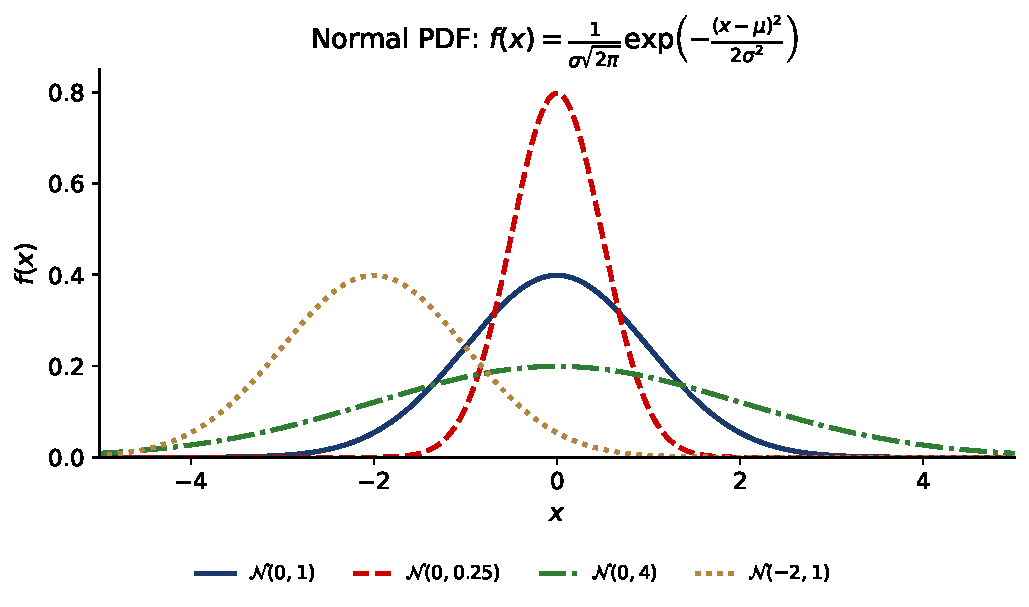
\includegraphics[width=\textwidth]{ch2_normal_pdf_theoretical.pdf}
            {\tiny Distribuția normală: simetrică, cozi exponențiale}
        \end{column}
    \end{columns}
\end{cminipage}
\end{frame}

\begin{frame}{Student-$t$: Efectul Gradelor de Libertate $\nu$}
\begin{cminipage}{0.95\textwidth}
    \begin{columns}[T]
        \begin{column}{0.52\textwidth}
            \begin{itemize}\setlength{\itemsep}{0pt}
                \item \textbf{Cum $\nu$ controlează forma distribuției:}
            \end{itemize}

            \vspace{0.1cm}
            \small
            \renewcommand{\arraystretch}{1.1}
            \begin{tabular}{cccc}
            \toprule
            $\nu$ & \textbf{Varianță} & \textbf{Kurtosis} & \textbf{Cozi} \\
            \midrule
            1 (Cauchy) & $\infty$ & $\infty$ & Foarte grele \\
            3 & 3.0 & $\infty$ & Grele \\
            5 & 1.67 & 9.0 & Moderate \\
            10 & 1.25 & 4.0 & Ușoare \\
            30 & 1.07 & 3.2 & $\approx$ Normal \\
            $\infty$ & 1.00 & 3.0 & Normal \\
            \bottomrule
            \end{tabular}
            \normalsize

            \vspace{0.2cm}
            \begin{itemize}\setlength{\itemsep}{0pt}
                \item \textbf{Randamente financiare:} $\hat{\nu} \approx 3$--$8$
                \item Cu cât $\nu$ mai mic, cu atât mai multe evenimente extreme
            \end{itemize}
        \end{column}
        \begin{column}{0.45\textwidth}
            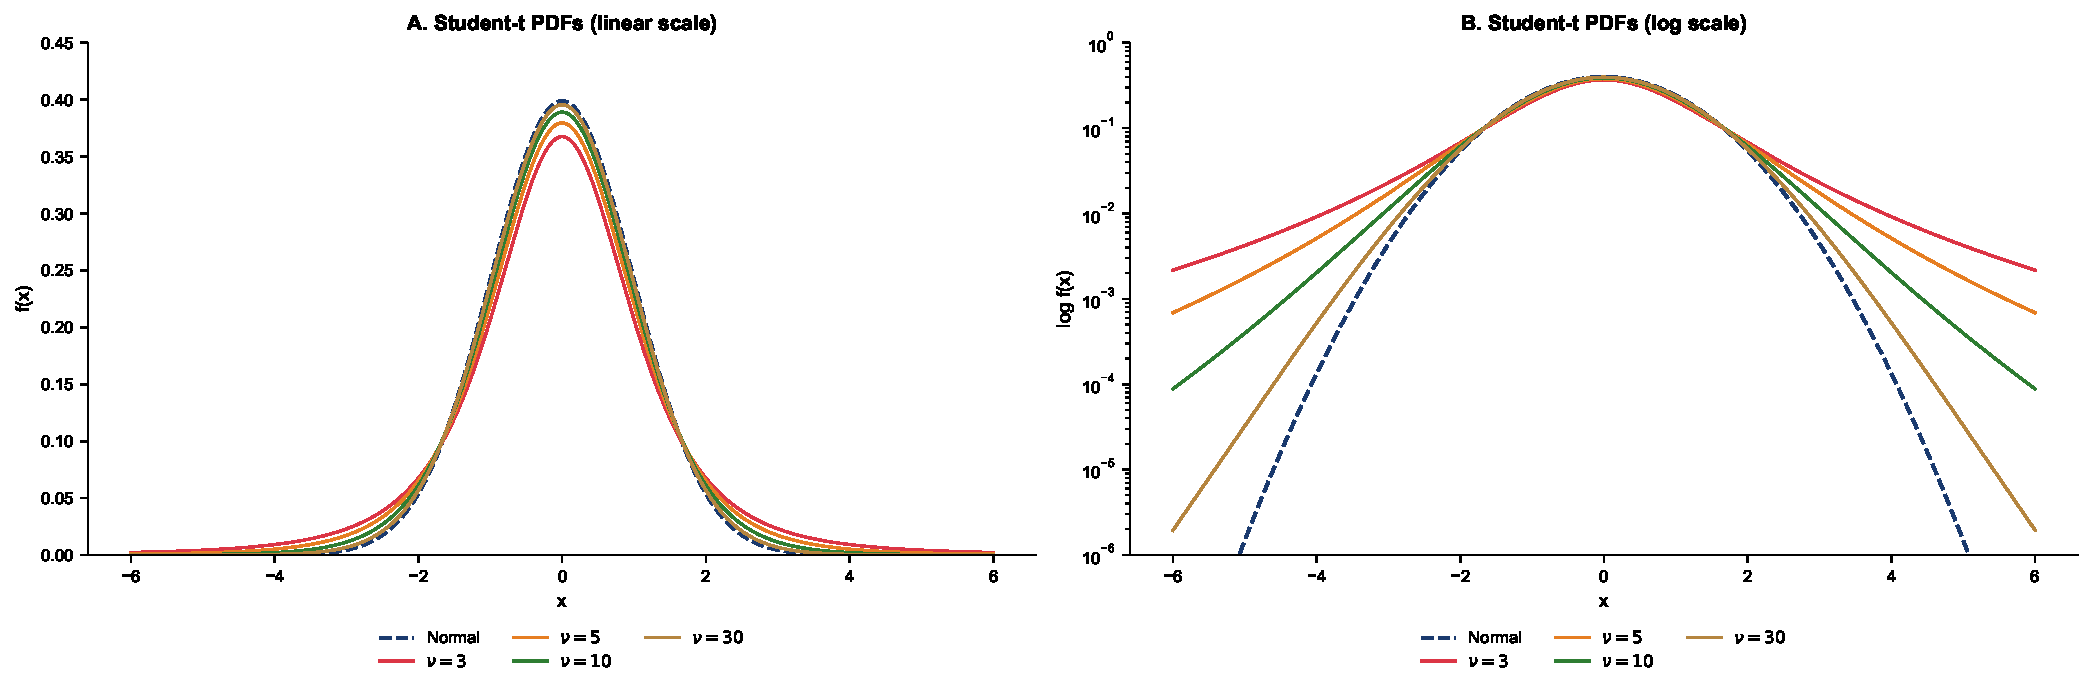
\includegraphics[width=\textwidth]{ch2_student_t_pdfs.pdf}
            {\tiny Student-$t$: de la Cauchy ($\nu=1$) la Normal ($\nu=\infty$)}
        \end{column}
    \end{columns}
\end{cminipage}
\end{frame}

\begin{frame}{Distribuția Pareto și Legea de Putere}
\begin{cminipage}{0.95\textwidth}
    \begin{columns}[T]
        \begin{column}{0.52\textwidth}
            \begin{itemize}\setlength{\itemsep}{0pt}
                \item \textbf{Legea de putere:} $\Pr(X > x) \sim x^{-\alpha}$
                \item \textbf{Declin polinomial} vs exponențial (Normal)
                \item Cozile sunt \textbf{mult} mai groase
            \end{itemize}

            \vspace{0.2cm}

            \begin{itemize}\setlength{\itemsep}{0pt}
                \item \textbf{Aplicații în finanțe:}
                \item Pierderi extreme (cozile randamentelor)
                \item Distribuția bogăției (regula 80/20)
                \item Volumele de tranzacționare
                \item Dimensiunea companiilor pe bursă
            \end{itemize}

            \vspace{0.2cm}

            \begin{itemize}\setlength{\itemsep}{0pt}
                \item \textbf{Proprietate cheie (scalabilitate):}
                \item $\Pr(X > 2x \mid X > x) = 2^{-\alpha}$, constant în $x$
                \item Probabilitatea condițională nu depinde de prag!
            \end{itemize}
        \end{column}
        \begin{column}{0.45\textwidth}
            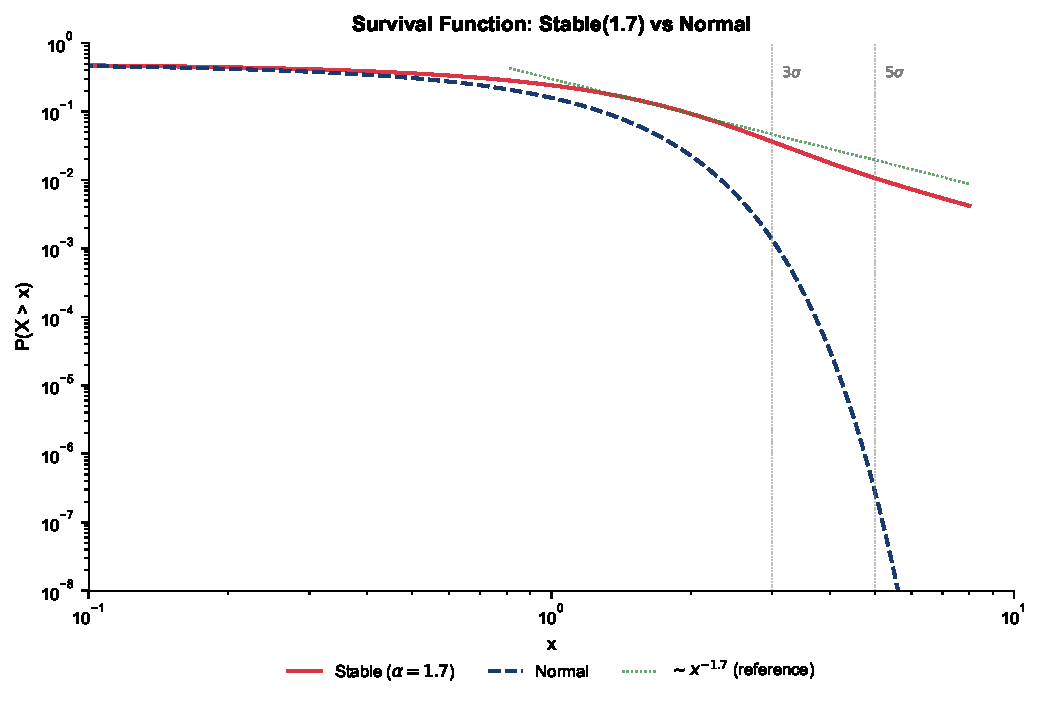
\includegraphics[width=\textwidth]{ch2_tail_survival.pdf}
            {\tiny Pareto: declin polinomial pe log-log}
        \end{column}
    \end{columns}
\end{cminipage}
\end{frame}

\begin{frame}{Comparație: Cozile Distribuțiilor}
\begin{cminipage}{0.95\textwidth}
    \begin{itemize}\setlength{\itemsep}{0pt}
        \item \textbf{Rata de declin a cozilor --- de la ușoare la grele:}
    \end{itemize}

    \vspace{0.2cm}
    \small
    \renewcommand{\arraystretch}{1.3}
    \begin{tabular}{lllll}
    \toprule
    \textbf{Distribuție} & \textbf{Declin coadă} & \textbf{Momente finite} & \textbf{VaR 1\%} ($\sigma=1\%$) & \textbf{Utilizare} \\
    \midrule
    Normal & $e^{-x^2/2}$ & Toate & 2.33\% & Benchmark \\
    Student-$t$ ($\nu=5$) & $x^{-(\nu+1)}$ & $p < \nu$ & 3.37\% & Randamente zilnice \\
    Pareto ($\alpha=3$) & $x^{-\alpha}$ & $p < \alpha$ & 9.28\% & Pierderi extreme \\
    Cauchy ($\nu=1$) & $x^{-2}$ & Niciun moment & -- & Caz limită \\
    \bottomrule
    \end{tabular}
    \normalsize

    \vspace{0.3cm}
    \begin{itemize}\setlength{\itemsep}{0pt}
        \item $\Rightarrow$ Cu cât cozile sunt mai grele, cu atât VaR crește \textbf{dramatic}
        \item Diferența este mică la 5\%, dar \textbf{enormă} la 0.1\%
        \item Alegerea distribuției contează cel mai mult în \textbf{cozile extreme}
    \end{itemize}
\end{cminipage}
\end{frame}

%=============================================================================
% PART 2: MULTIPLE CHOICE QUIZZES
%=============================================================================
\section{Test Grilă}

\begin{frame}{Test 1: Testul Jarque--Bera}
\begin{cminipage}{0.95\textwidth}
    \begin{alertblock}{Întrebare}
        Testul Jarque--Bera verifică:
    \end{alertblock}

    \vspace{0.5cm}
    \begin{block}{Variante de răspuns}
    \textcolor{MainBlue}{\textbf{(A)}} Staționaritatea seriei\\[3pt]
    \textcolor{MainBlue}{\textbf{(B)}} Normalitatea distribuției\\[3pt]
    \textcolor{MainBlue}{\textbf{(C)}} Absența autocorelației\\[3pt]
    \textcolor{MainBlue}{\textbf{(D)}} Homoscedasticitatea
    \end{block}
\end{cminipage}
\end{frame}

\begin{frame}{Test 1: Răspuns}
\begin{cminipage}{0.95\textwidth}
    \begin{columns}[T]
        \begin{column}{0.52\textwidth}
            \begin{exampleblock}{Răspuns: B}
                Normalitatea distribuției
            \end{exampleblock}

            \vspace{0.2cm}

            \begin{itemize}\setlength{\itemsep}{0pt}
                \item \textbf{Explicație:}
            \end{itemize}
            $$JB = \frac{n}{6}\left(\hat{S}^2 + \frac{(\hat{K} - 3)^2}{4}\right) \sim \chi^2(2)$$

            \begin{itemize}\setlength{\itemsep}{0pt}
                \item $H_0$: Distribuția este normală ($S=0$, $K=3$)
                \item $H_1$: Distribuția nu este normală
                \item Se bazează pe skewness și kurtosis
            \end{itemize}
        \end{column}
        \begin{column}{0.45\textwidth}
            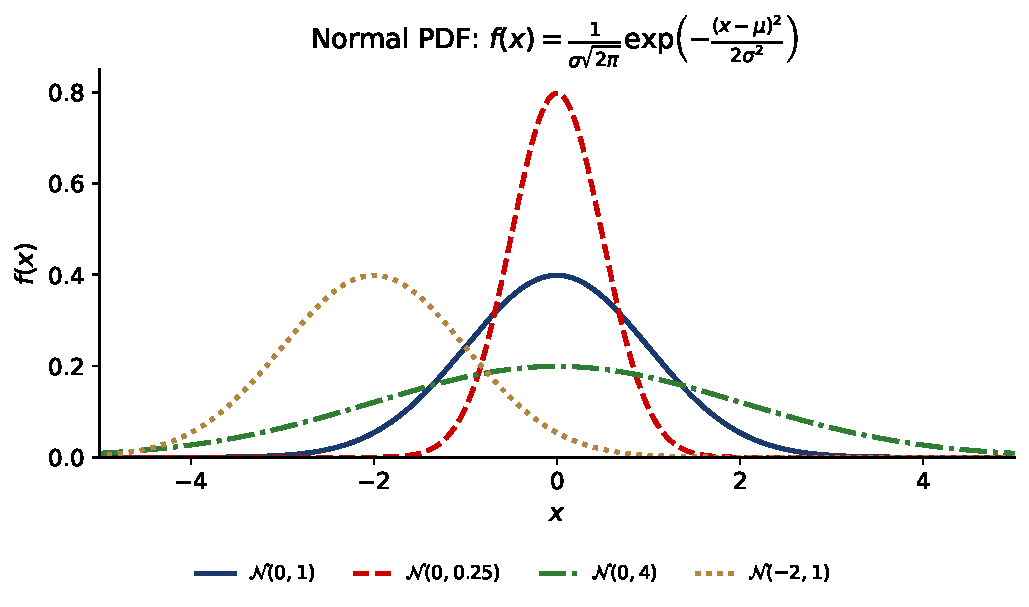
\includegraphics[width=\textwidth]{ch2_normal_pdf_theoretical.pdf}
            {\tiny Distribuția normală: $S=0$, $K=3$}
        \end{column}
    \end{columns}
    \quantlet{SFM\_ch2\_normal\_distribution}{https://github.com/QuantLet/Stat_fin_markets/tree/master/Ch_02/SFM_ch2_normal_distribution}
\end{cminipage}
\end{frame}

\begin{frame}{Test 2: Excesul de kurtosis}
\begin{cminipage}{0.95\textwidth}
    \begin{alertblock}{Întrebare}
        Excesul de kurtosis al distribuției Student-$t$ cu $\nu = 6$ este:
    \end{alertblock}

    \vspace{0.5cm}
    \begin{block}{Variante de răspuns}
    \textcolor{MainBlue}{\textbf{(A)}} 1.5\\[3pt]
    \textcolor{MainBlue}{\textbf{(B)}} 3.0\\[3pt]
    \textcolor{MainBlue}{\textbf{(C)}} 6.0\\[3pt]
    \textcolor{MainBlue}{\textbf{(D)}} Nu există
    \end{block}
\end{cminipage}
\end{frame}

\begin{frame}{Test 2: Răspuns}
\begin{cminipage}{0.95\textwidth}
    \begin{columns}[T]
        \begin{column}{0.52\textwidth}
            \begin{exampleblock}{Răspuns: B}
                $\kappa = 6/(6-4) = 3.0$
            \end{exampleblock}

            \vspace{0.2cm}

            \begin{itemize}\setlength{\itemsep}{0pt}
                \item \textbf{Formula excesului de kurtosis:}
            \end{itemize}
            $$\kappa = \frac{6}{\nu - 4} \quad \text{pentru } \nu > 4$$

            \begin{itemize}\setlength{\itemsep}{0pt}
                \item Verificarea opțiunilor:
                \item A: $\kappa = 1.5$ ar necesita $\nu = 8$ \incorrect
                \item B: $\kappa = 6/(6-4) = 3.0$ \correct
                \item C: $\kappa = 6.0$ ar necesita $\nu = 5$ \incorrect
                \item D: Kurtosis există pentru $\nu > 4$ \incorrect
            \end{itemize}
        \end{column}
        \begin{column}{0.45\textwidth}
            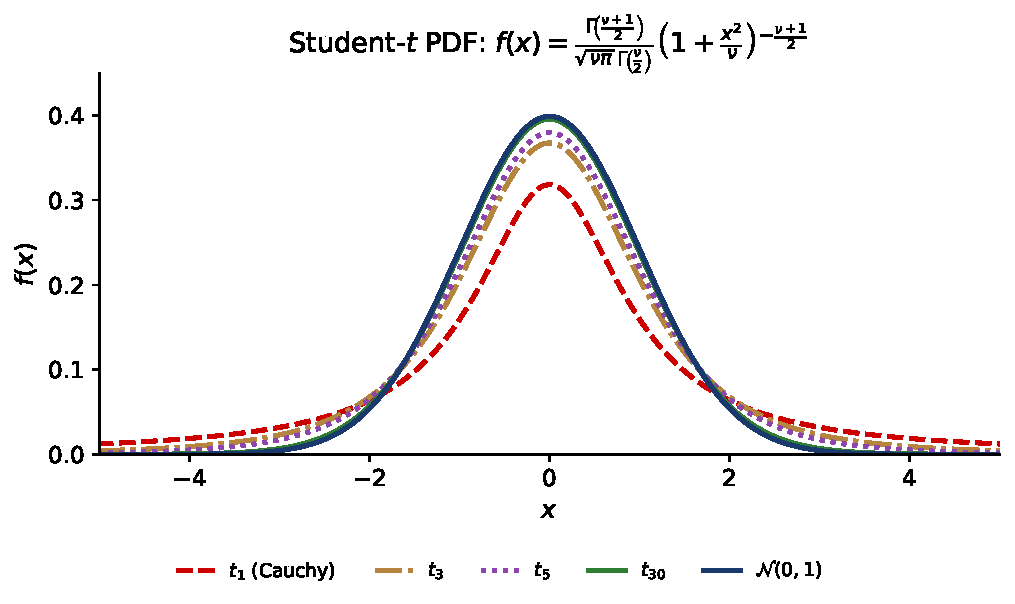
\includegraphics[width=\textwidth]{ch2_student_t_pdf_theoretical.pdf}
            {\tiny Student-$t$: cozi grele, $\kappa > 0$}
        \end{column}
    \end{columns}
    \quantlet{SFM\_ch2\_student\_t}{https://github.com/QuantLet/Stat_fin_markets/tree/master/Ch_02/SFM_ch2_student_t}
\end{cminipage}
\end{frame}

\begin{frame}{Test 3: VaR Normal}
\begin{cminipage}{0.95\textwidth}
    \begin{alertblock}{Întrebare}
        VaR Normal la 1\% cu $\mu = 0$, $\sigma = 1\%$ este aproximativ:
    \end{alertblock}

    \vspace{0.5cm}
    \begin{block}{Variante de răspuns}
    \textcolor{MainBlue}{\textbf{(A)}} 1.65\%\\[3pt]
    \textcolor{MainBlue}{\textbf{(B)}} 2.33\%\\[3pt]
    \textcolor{MainBlue}{\textbf{(C)}} 3.09\%\\[3pt]
    \textcolor{MainBlue}{\textbf{(D)}} 3.72\%
    \end{block}
\end{cminipage}
\end{frame}

\begin{frame}{Test 3: Răspuns}
\begin{cminipage}{0.95\textwidth}
    \begin{columns}[T]
        \begin{column}{0.52\textwidth}
            \begin{exampleblock}{Răspuns: B}
                $\text{VaR}_{1\%} = 2.326 \times 1\% \approx 2.33\%$
            \end{exampleblock}

            \vspace{0.2cm}

            \begin{itemize}\setlength{\itemsep}{0pt}
                \item \textbf{Formula VaR Normal:}
            \end{itemize}
            $$\text{VaR}_\alpha = -(\mu + z_\alpha \cdot \sigma)$$

            \begin{itemize}\setlength{\itemsep}{0pt}
                \item Cuantilele cheie:
                \item A: $z_{5\%} = -1.645$ \incorrect
                \item B: $z_{1\%} = -2.326$ \correct
                \item C: $z_{0.1\%} = -3.090$ \incorrect
                \item D: Nu corespunde unui nivel standard \incorrect
            \end{itemize}
        \end{column}
        \begin{column}{0.45\textwidth}
            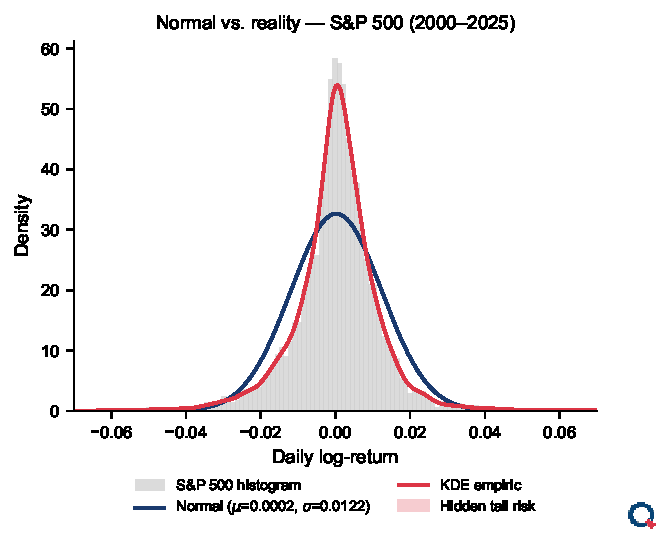
\includegraphics[width=\textwidth]{ch2_normal_vs_empirical.pdf}
            {\tiny VaR: cuantila stângă a distribuției}
        \end{column}
    \end{columns}
    \quantlet{SFM\_ch2\_risk\_management}{https://github.com/QuantLet/Stat_fin_markets/tree/master/Ch_02/SFM_ch2_risk_management}
\end{cminipage}
\end{frame}

\begin{frame}{Test 4: Student-$t$ și convergența}
\begin{cminipage}{0.95\textwidth}
    \begin{alertblock}{Întrebare}
        Când $\nu \to \infty$, distribuția Student-$t$:
    \end{alertblock}

    \vspace{0.5cm}
    \begin{block}{Variante de răspuns}
    \textcolor{MainBlue}{\textbf{(A)}} Converge la Cauchy\\[3pt]
    \textcolor{MainBlue}{\textbf{(B)}} Converge la Normal\\[3pt]
    \textcolor{MainBlue}{\textbf{(C)}} Varianța devine infinită\\[3pt]
    \textcolor{MainBlue}{\textbf{(D)}} Nu converge
    \end{block}
\end{cminipage}
\end{frame}

\begin{frame}{Test 4: Răspuns}
\begin{cminipage}{0.95\textwidth}
    \begin{columns}[T]
        \begin{column}{0.52\textwidth}
            \begin{exampleblock}{Răspuns: B}
                Converge la distribuția normală standard
            \end{exampleblock}

            \vspace{0.2cm}

            \begin{itemize}\setlength{\itemsep}{0pt}
                \item \textbf{Ierarhia distribuțiilor:}
                \item $\nu = 1$: Cauchy (cozi foarte grele)
                \item $\nu = 3$--$8$: randamente financiare tipice
                \item $\nu = 30$: aproape normală
                \item $\nu \to \infty$: exact $\mathcal{N}(0,1)$
                \item $\Rightarrow$ Distribuția normală este un \textbf{caz limită} al Student-$t$.
            \end{itemize}
        \end{column}
        \begin{column}{0.45\textwidth}
            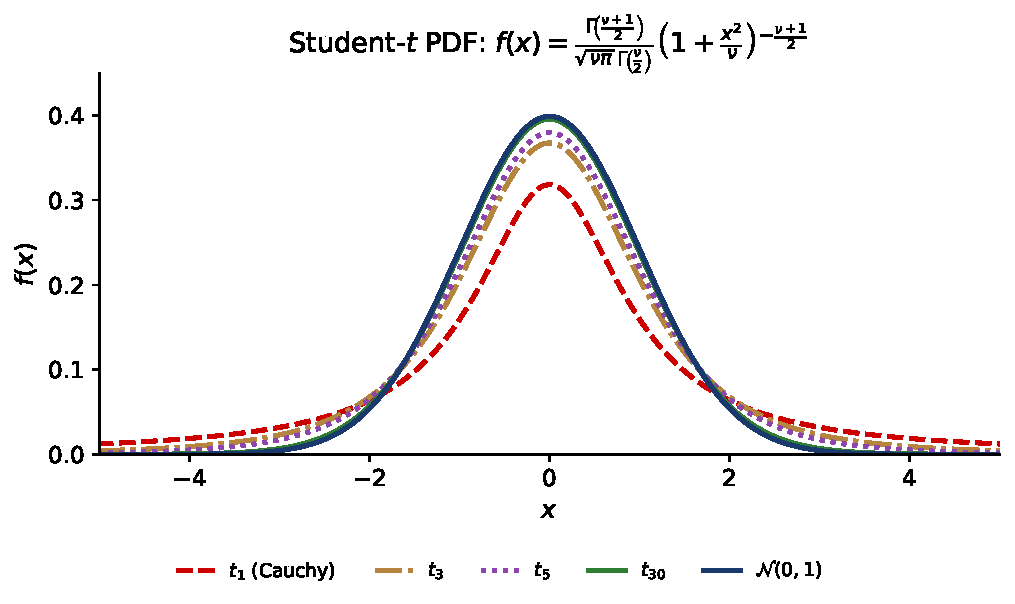
\includegraphics[width=\textwidth]{ch2_student_t_pdf_theoretical.pdf}
            {\tiny Student-$t$ converge la normal pe măsură ce $\nu \to \infty$}
        \end{column}
    \end{columns}
    \quantlet{SFM\_ch2\_student\_t}{https://github.com/QuantLet/Stat_fin_markets/tree/master/Ch_02/SFM_ch2_student_t}
\end{cminipage}
\end{frame}

\begin{frame}{Test 5: Expected Shortfall}
\begin{cminipage}{0.95\textwidth}
    \begin{alertblock}{Întrebare}
        Care afirmație despre ES este \textbf{adevărată}?
    \end{alertblock}

    \vspace{0.5cm}
    \begin{block}{Variante de răspuns}
    \textcolor{MainBlue}{\textbf{(A)}} $\text{ES} < \text{VaR}$ întotdeauna\\[3pt]
    \textcolor{MainBlue}{\textbf{(B)}} $\text{ES} \geq \text{VaR}$ întotdeauna\\[3pt]
    \textcolor{MainBlue}{\textbf{(C)}} $\text{ES} = \text{VaR}$ sub normalitate\\[3pt]
    \textcolor{MainBlue}{\textbf{(D)}} ES nu este definit sub Student-$t$
    \end{block}
\end{cminipage}
\end{frame}

\begin{frame}{Test 5: Răspuns}
\begin{cminipage}{0.95\textwidth}
    \begin{columns}[T]
        \begin{column}{0.52\textwidth}
            \begin{exampleblock}{Răspuns: B}
                $\text{ES} \geq \text{VaR}$ întotdeauna
            \end{exampleblock}

            \vspace{0.2cm}

            \begin{itemize}\setlength{\itemsep}{0pt}
                \item \textbf{Definiția ES:}
            \end{itemize}
            $$\text{ES}_\alpha = \E[-X \mid -X > \text{VaR}_\alpha]$$

            \begin{itemize}\setlength{\itemsep}{0pt}
                \item ES este media pierderilor \textit{condiționate} de depășirea VaR $\Rightarrow$ nu poate fi mai mică decât VaR.
                \item Sub normalitate: $\text{ES}/\text{VaR} \approx 1.14$ la 1\%.
                \item Sub Student-$t$: raportul crește cu scăderea $\nu$.
            \end{itemize}
        \end{column}
        \begin{column}{0.45\textwidth}
            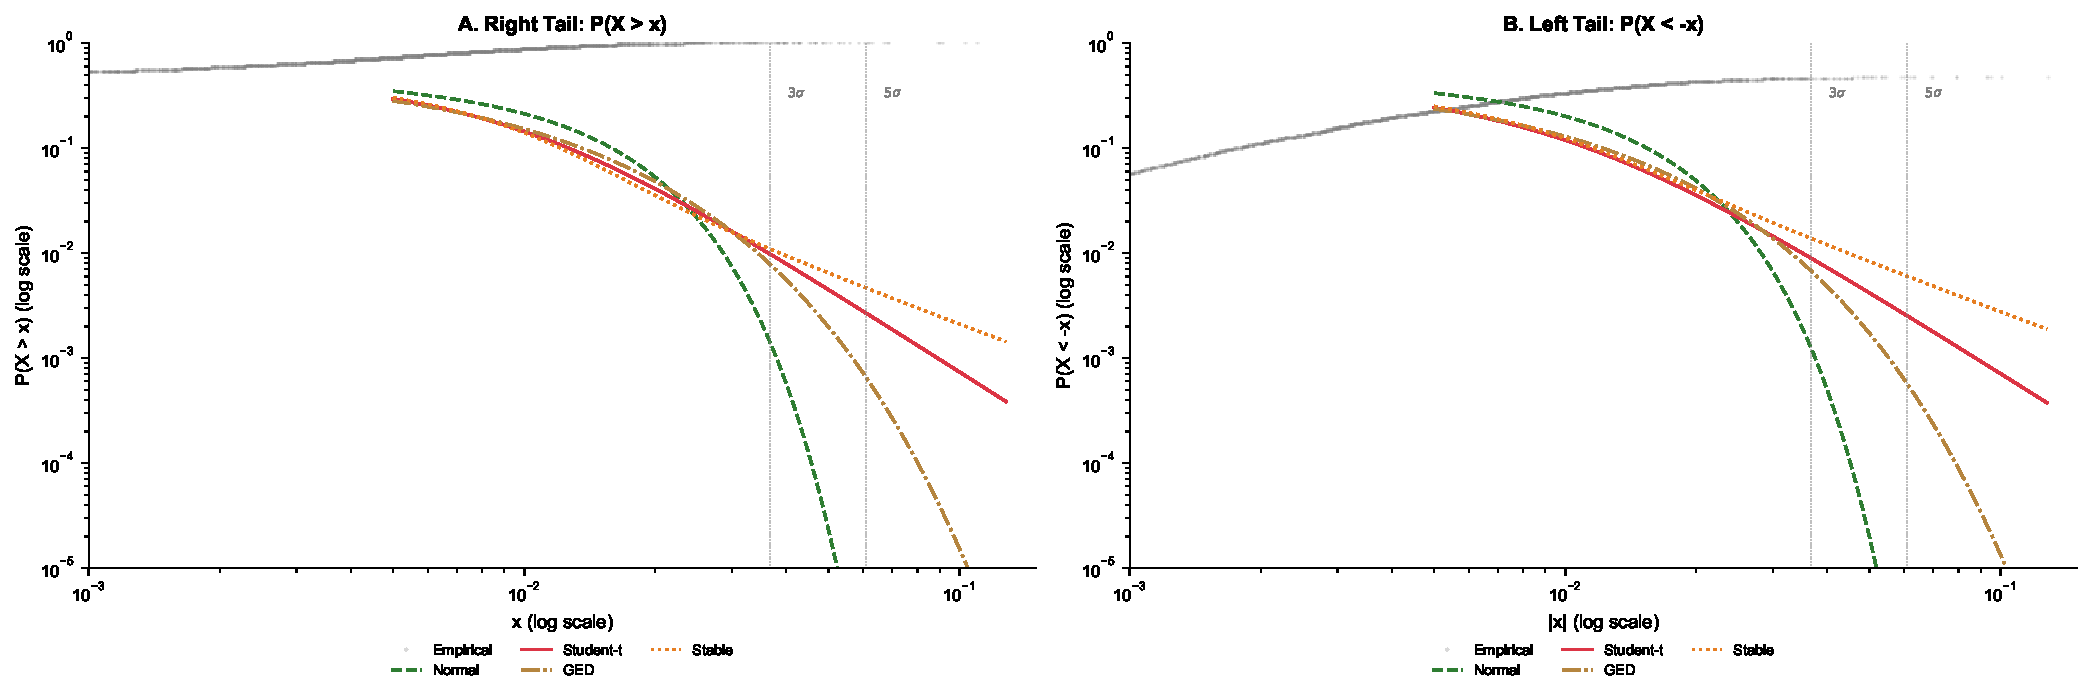
\includegraphics[width=\textwidth]{ch2_dist_comparison_tails.pdf}
            {\tiny ES: aria sub coadă dincolo de VaR}
        \end{column}
    \end{columns}
    \quantlet{SFM\_ch2\_risk\_management}{https://github.com/QuantLet/Stat_fin_markets/tree/master/Ch_02/SFM_ch2_risk_management}
\end{cminipage}
\end{frame}

\begin{frame}{Test 6: Faptele stilizate}
\begin{cminipage}{0.95\textwidth}
    \begin{alertblock}{Întrebare}
        Care dintre următoarele NU este un fapt stilizat al randamentelor financiare?
    \end{alertblock}

    \vspace{0.5cm}
    \begin{block}{Variante de răspuns}
    \textcolor{MainBlue}{\textbf{(A)}} Cozi grele (leptokurtosis)\\[3pt]
    \textcolor{MainBlue}{\textbf{(B)}} Volatility clustering\\[3pt]
    \textcolor{MainBlue}{\textbf{(C)}} Distribuție normală perfectă\\[3pt]
    \textcolor{MainBlue}{\textbf{(D)}} Asimetrie negativă
    \end{block}
\end{cminipage}
\end{frame}

\begin{frame}{Test 6: Răspuns}
\begin{cminipage}{0.95\textwidth}
    \begin{columns}[T]
        \begin{column}{0.52\textwidth}
            \begin{exampleblock}{Răspuns: C}
                Randamentele reale NU sunt normal distribuite
            \end{exampleblock}

            \vspace{0.2cm}

            \begin{itemize}\setlength{\itemsep}{0pt}
                \item \textbf{Faptele stilizate (Cont, 2001):}
                \item Cozi grele: $\hat{K} > 3$ \correct
                \item Volatility clustering \correct
                \item Asimetrie negativă pe acțiuni \correct
                \item Normalitate: \textcolor{Crimson}{respinsă} pe toate piețele \incorrect
                \item $\Rightarrow$ Normalitatea este o \textbf{aproximare}, nu un fapt.
            \end{itemize}
        \end{column}
        \begin{column}{0.45\textwidth}
            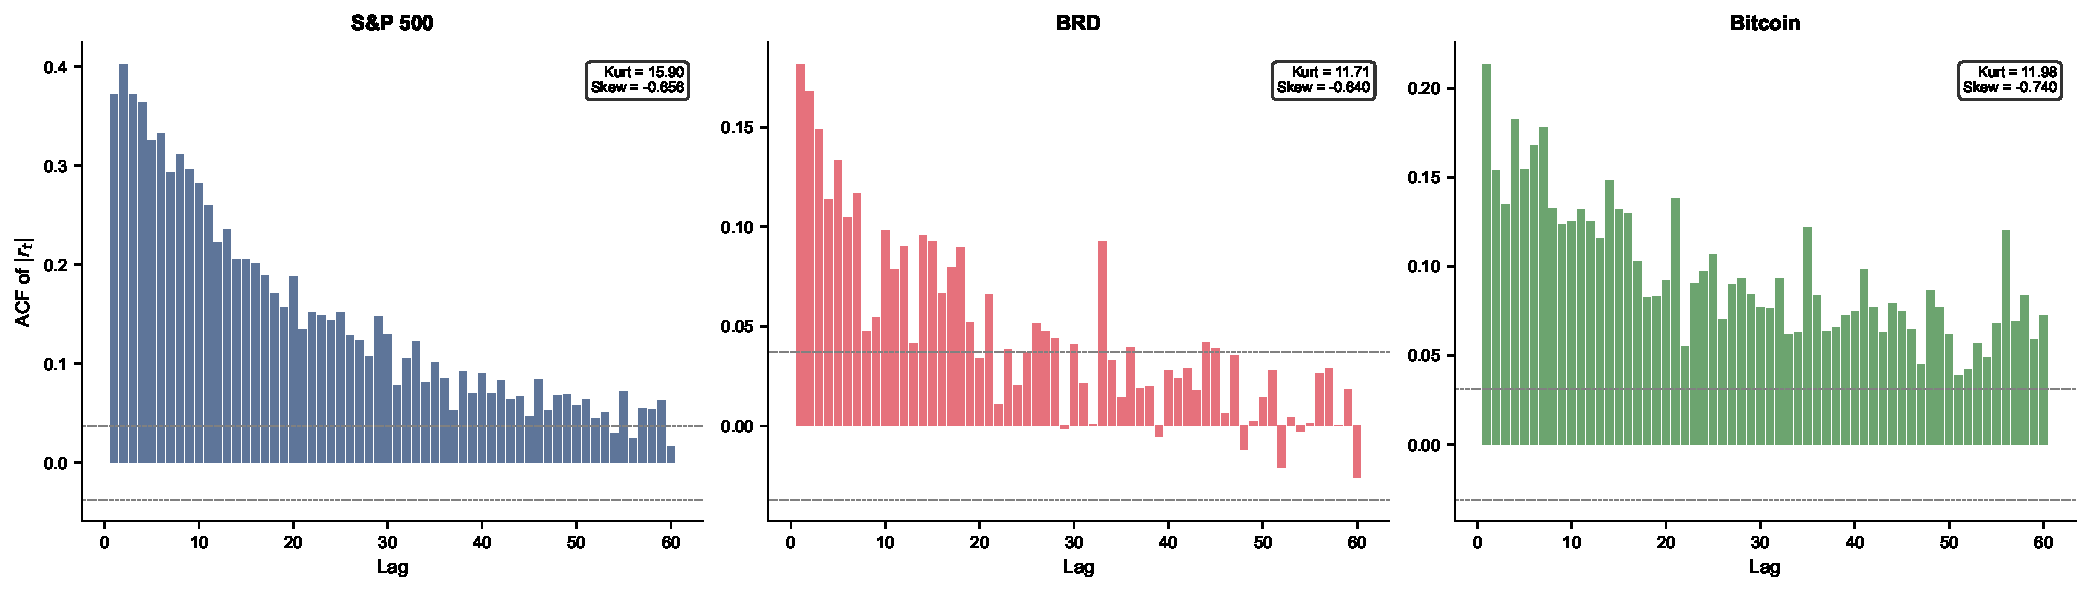
\includegraphics[width=\textwidth]{ch2_cs2a_stylized_3assets.pdf}
            {\tiny Fapte stilizate: comparație 3 active}
        \end{column}
    \end{columns}
    \quantlet{SFM\_ch2\_case\_study\_2a}{https://github.com/QuantLet/Stat_fin_markets/tree/master/Ch_02/SFM_ch2_case_study_2a}
\end{cminipage}
\end{frame}

\begin{frame}{Test 7: Skewness-ul randamentelor}
\begin{cminipage}{0.95\textwidth}
    \begin{alertblock}{Întrebare}
        Pe randamente zilnice de acțiuni, $\hat{S} = -0.5$ sugerează:
    \end{alertblock}

    \vspace{0.5cm}
    \begin{block}{Variante de răspuns}
    \textcolor{MainBlue}{\textbf{(A)}} Mai multe randamente pozitive extreme\\[3pt]
    \textcolor{MainBlue}{\textbf{(B)}} Mai multe randamente negative extreme\\[3pt]
    \textcolor{MainBlue}{\textbf{(C)}} Simetrie perfectă\\[3pt]
    \textcolor{MainBlue}{\textbf{(D)}} Kurtosis excesivă
    \end{block}
\end{cminipage}
\end{frame}

\begin{frame}{Test 7: Răspuns}
\begin{cminipage}{0.95\textwidth}
    \begin{columns}[T]
        \begin{column}{0.52\textwidth}
            \begin{exampleblock}{Răspuns: B}
                Coada stângă este mai grea
            \end{exampleblock}

            \vspace{0.2cm}

            \begin{itemize}\setlength{\itemsep}{0pt}
                \item \textbf{Interpretarea skewness:}
                \item $S < 0$: coada stângă mai lungă (pierderi mari) \correct
                \item $S > 0$: coada dreaptă mai lungă
                \item $S = 0$: simetrie
                \item Pe acțiuni: efectul de \textbf{levier} (Black, 1976) --- scăderile sunt mai abrupte decât creșterile.
            \end{itemize}
        \end{column}
        \begin{column}{0.45\textwidth}
            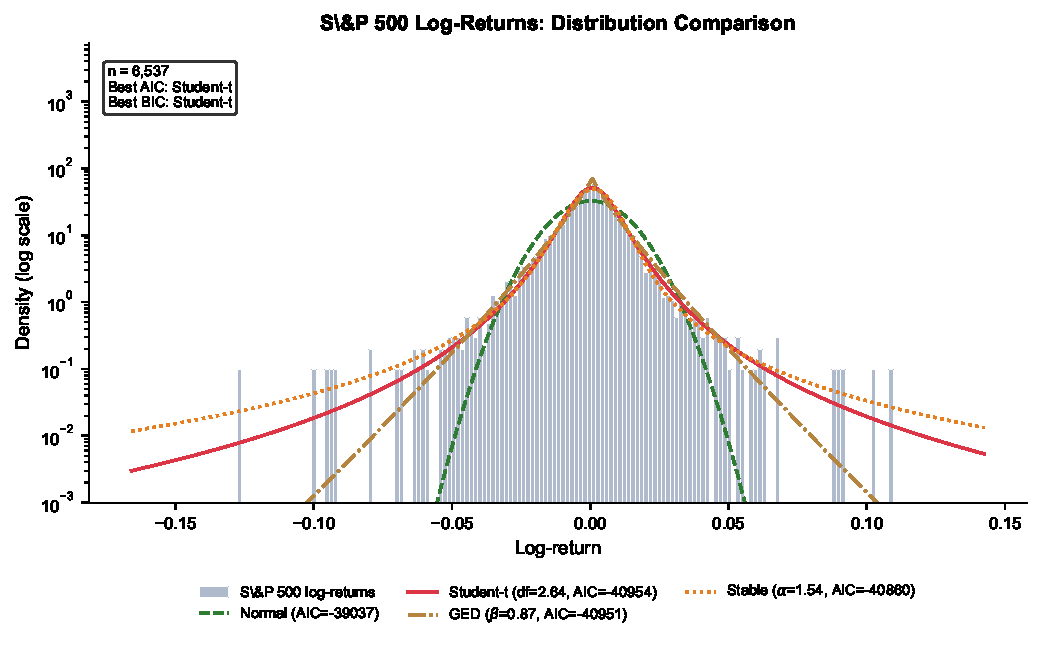
\includegraphics[width=\textwidth]{ch2_dist_comparison_overlay.pdf}
            {\tiny Skewness negativ: coada stângă mai grea}
        \end{column}
    \end{columns}
    \quantlet{SFM\_ch2\_distribution\_comparison}{https://github.com/QuantLet/Stat_fin_markets/tree/master/Ch_02/SFM_ch2_distribution_comparison}
\end{cminipage}
\end{frame}

\begin{frame}{Test 8: MLE pentru Normal}
\begin{cminipage}{0.95\textwidth}
    \begin{alertblock}{Întrebare}
        Estimatorul MLE pentru $\sigma^2$ în cazul normal este:
    \end{alertblock}

    \vspace{0.5cm}
    \begin{block}{Variante de răspuns}
    \textcolor{MainBlue}{\textbf{(A)}} $\frac{1}{n-1}\sum_{i=1}^n(x_i - \bar{x})^2$\\[3pt]
    \textcolor{MainBlue}{\textbf{(B)}} $\frac{1}{n}\sum_{i=1}^n(x_i - \bar{x})^2$\\[3pt]
    \textcolor{MainBlue}{\textbf{(C)}} $\frac{1}{n}\sum_{i=1}^n x_i^2$\\[3pt]
    \textcolor{MainBlue}{\textbf{(D)}} $\frac{1}{n-2}\sum_{i=1}^n(x_i - \bar{x})^2$
    \end{block}
\end{cminipage}
\end{frame}

\begin{frame}{Test 8: Răspuns}
\begin{cminipage}{0.95\textwidth}
    \begin{columns}[T]
        \begin{column}{0.52\textwidth}
            \begin{exampleblock}{Răspuns: B}
                $\hat{\sigma}^2_{\text{MLE}} = \frac{1}{n}\sum(x_i - \bar{x})^2$
            \end{exampleblock}

            \vspace{0.2cm}

            \begin{itemize}\setlength{\itemsep}{0pt}
                \item \textbf{Explicație:}
                \item MLE maximizează log-verosimilitatea:
            \end{itemize}
            $$\ell(\mu,\sigma^2) = -\frac{n}{2}\ln(2\pi\sigma^2) - \frac{1}{2\sigma^2}\sum(x_i-\mu)^2$$

            \begin{itemize}\setlength{\itemsep}{0pt}
                \item A: estimatorul nedeplasat (corect, dar nu MLE) \incorrect
                \item B: MLE (ușor deplasat) \correct
                \item C: nu centrează la medie \incorrect
            \end{itemize}
        \end{column}
        \begin{column}{0.45\textwidth}
            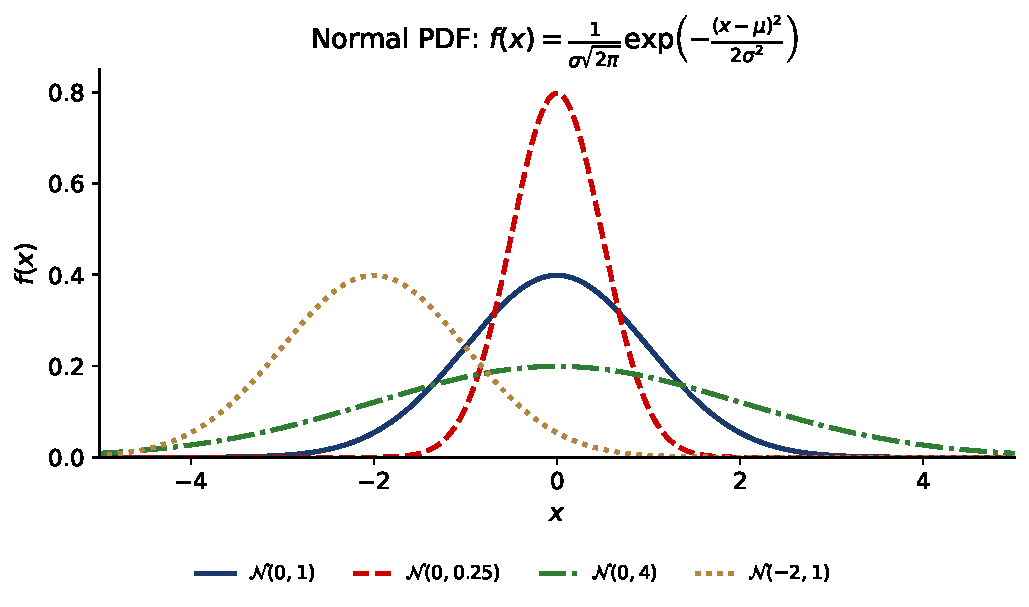
\includegraphics[width=\textwidth]{ch2_normal_pdf_theoretical.pdf}
            {\tiny Normal: MLE coincide cu momentele}
        \end{column}
    \end{columns}
    \quantlet{SFM\_ch2\_normal\_distribution}{https://github.com/QuantLet/Stat_fin_markets/tree/master/Ch_02/SFM_ch2_normal_distribution}
\end{cminipage}
\end{frame}

\begin{frame}{Test 9: Raportul ES/VaR}
\begin{cminipage}{0.95\textwidth}
    \begin{alertblock}{Întrebare}
        Dacă VaR la 1\% = 3\% și ES la 1\% = 4.5\%, raportul ES/VaR este:
    \end{alertblock}

    \vspace{0.5cm}
    \begin{block}{Variante de răspuns}
    \textcolor{MainBlue}{\textbf{(A)}} 0.67\\[3pt]
    \textcolor{MainBlue}{\textbf{(B)}} 1.00\\[3pt]
    \textcolor{MainBlue}{\textbf{(C)}} 1.50\\[3pt]
    \textcolor{MainBlue}{\textbf{(D)}} 3.00
    \end{block}
\end{cminipage}
\end{frame}

\begin{frame}{Test 9: Răspuns}
\begin{cminipage}{0.95\textwidth}
    \begin{columns}[T]
        \begin{column}{0.52\textwidth}
            \begin{exampleblock}{Răspuns: C}
                ES/VaR = 4.5\%/3\% = 1.50
            \end{exampleblock}

            \vspace{0.2cm}

            \begin{itemize}\setlength{\itemsep}{0pt}
                \item \textbf{Raportul ES/VaR:}
                \item Sub normalitate la 1\%: $\approx 1.14$
                \item Sub Student-$t$($\nu = 5$) la 1\%: $\approx 1.50$
                \item Cu cât cozile sunt mai grele, cu atât raportul crește
                \item ES/VaR $= 1.50 > 1.14$ $\Rightarrow$ distribuția este mai grea decât distribuția normală.
            \end{itemize}
        \end{column}
        \begin{column}{0.45\textwidth}
            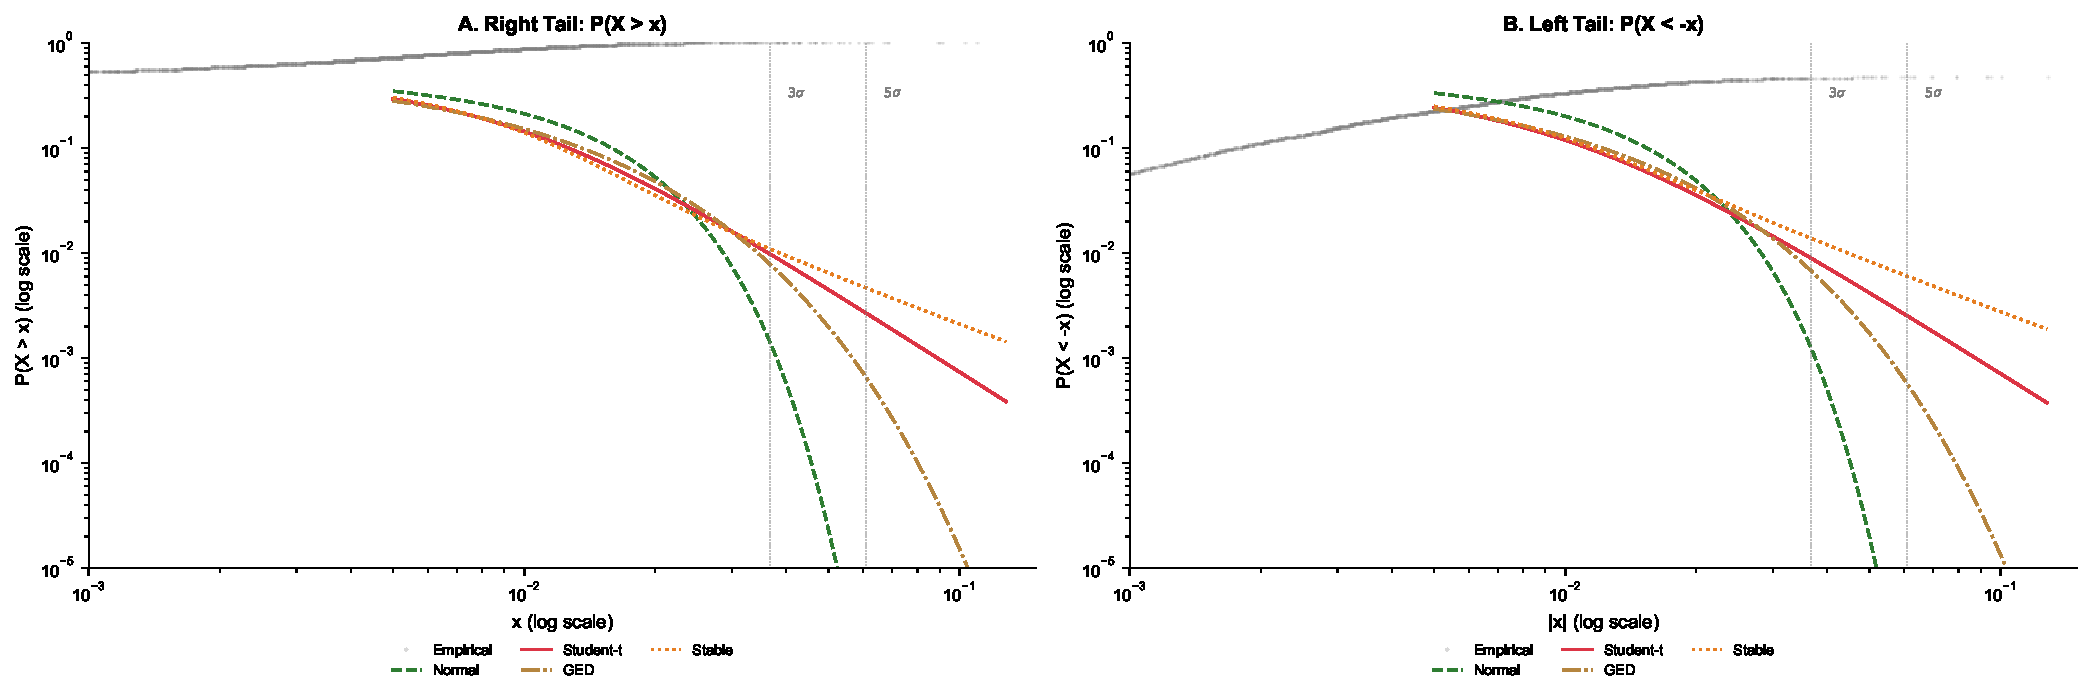
\includegraphics[width=\textwidth]{ch2_dist_comparison_tails.pdf}
            {\tiny ES captează severitatea pierderilor extreme}
        \end{column}
    \end{columns}
    \quantlet{SFM\_ch2\_distribution\_comparison}{https://github.com/QuantLet/Stat_fin_markets/tree/master/Ch_02/SFM_ch2_distribution_comparison}
\end{cminipage}
\end{frame}

\begin{frame}{Test 10: Penalizarea BIC}
\begin{cminipage}{0.95\textwidth}
    \begin{alertblock}{Întrebare}
        Pe un eșantion de $n = 5000$, BIC penalizează un parametru suplimentar cu:
    \end{alertblock}

    \vspace{0.5cm}
    \begin{block}{Variante de răspuns}
    \textcolor{MainBlue}{\textbf{(A)}} 2\\[3pt]
    \textcolor{MainBlue}{\textbf{(B)}} 8.52\\[3pt]
    \textcolor{MainBlue}{\textbf{(C)}} 5000\\[3pt]
    \textcolor{MainBlue}{\textbf{(D)}} $\ln(2) \approx 0.69$
    \end{block}
\end{cminipage}
\end{frame}

\begin{frame}{Test 10: Răspuns}
\begin{cminipage}{0.95\textwidth}
    \begin{columns}[T]
        \begin{column}{0.52\textwidth}
            \begin{exampleblock}{Răspuns: B}
                $\ln(5000) \approx 8.52$ per parametru
            \end{exampleblock}

            \vspace{0.2cm}

            \begin{itemize}\setlength{\itemsep}{0pt}
                \item \textbf{Comparație AIC vs BIC:}
            \end{itemize}
            \begin{align*}
                \text{AIC}&: \text{penalizare} = 2k \\
                \text{BIC}&: \text{penalizare} = k\ln(n)
            \end{align*}

            \begin{itemize}\setlength{\itemsep}{0pt}
                \item Pentru $n = 5000$:
                \item AIC: $+2$ per parametru
                \item BIC: $+8.52$ per parametru
                \item $\Rightarrow$ BIC favorizează modele \textbf{mai parcimonioase}.
            \end{itemize}
        \end{column}
        \begin{column}{0.45\textwidth}
            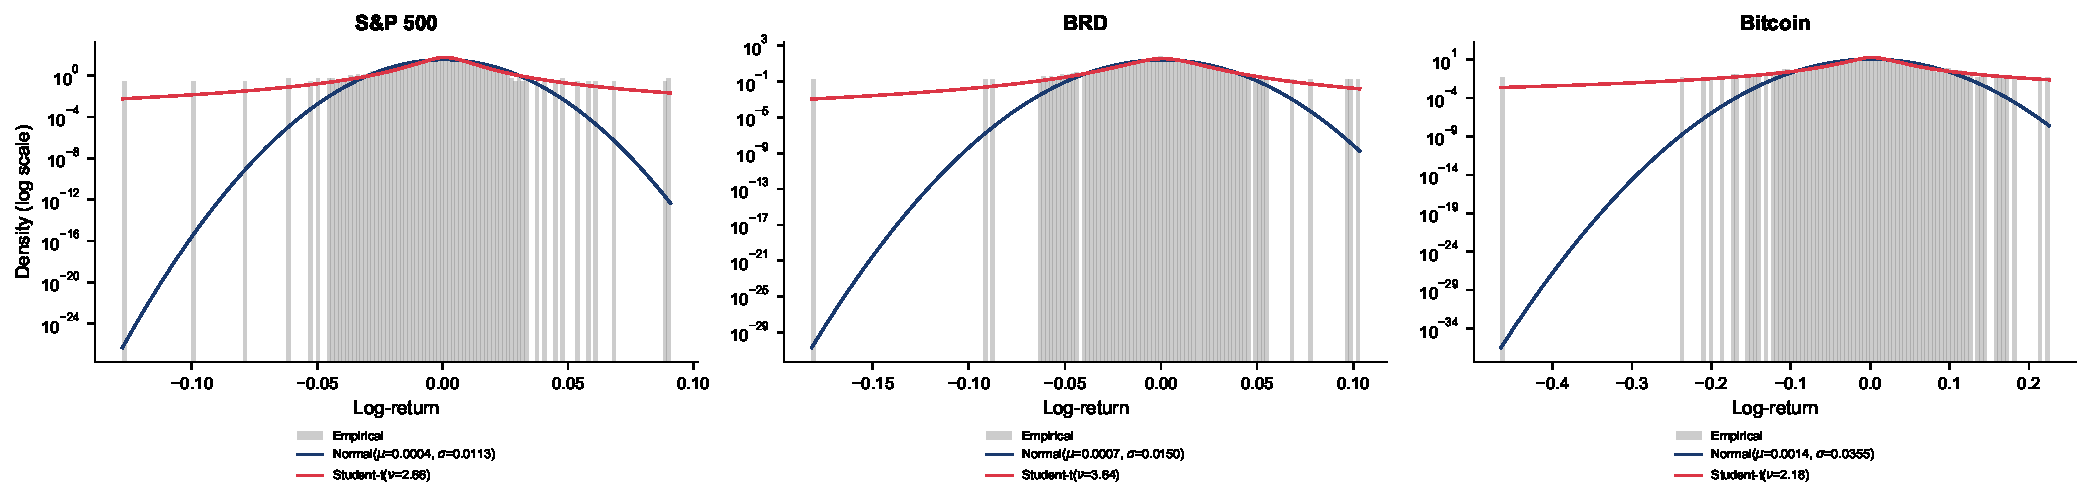
\includegraphics[width=\textwidth]{ch2_cs2a_fit_comparison.pdf}
            {\tiny AIC vs BIC: selecția modelului}
        \end{column}
    \end{columns}
    \quantlet{SFM\_ch2\_distribution\_comparison}{https://github.com/QuantLet/Stat_fin_markets/tree/master/Ch_02/SFM_ch2_distribution_comparison}
\end{cminipage}
\end{frame}

\begin{frame}{Test 11: Distribuția Pareto}
\begin{cminipage}{0.95\textwidth}
    \begin{alertblock}{Întrebare}
        Funcția de supraviețuire a distribuției Pareto($x_m, \alpha$) este:
    \end{alertblock}

    \vspace{0.5cm}
    \begin{block}{Variante de răspuns}
    \textcolor{MainBlue}{\textbf{(A)}} $\bar{F}(x) = (x_m / x)^{\alpha}$\\[3pt]
    \textcolor{MainBlue}{\textbf{(B)}} $\bar{F}(x) = e^{-\alpha x}$\\[3pt]
    \textcolor{MainBlue}{\textbf{(C)}} $\bar{F}(x) = 1/(1 + x^\alpha)$\\[3pt]
    \textcolor{MainBlue}{\textbf{(D)}} $\bar{F}(x) = (x/x_m)^{-\alpha}$
    \end{block}
\end{cminipage}
\end{frame}

\begin{frame}{Test 11: Răspuns}
\begin{cminipage}{0.95\textwidth}
    \begin{columns}[T]
        \begin{column}{0.52\textwidth}
            \begin{exampleblock}{Răspuns: A}
                $\bar{F}(x) = \Pr(X > x) = (x_m / x)^{\alpha}$ pentru $x \geq x_m$
            \end{exampleblock}

            \vspace{0.2cm}

            \begin{itemize}\setlength{\itemsep}{0pt}
                \item \textbf{Explicație:}
                \item A: Corect --- declin polinomial (legea de putere) \correct
                \item B: Declin exponențial (Exponențială, nu Pareto) \incorrect
                \item C: Distribuția log-logistică \incorrect
                \item D: Echivalent cu A doar dacă $x_m = 1$ \incorrect
                \item Cheia: cozile Pareto scad ca $x^{-\alpha}$, \textbf{mult mai lent} decât $e^{-x}$.
            \end{itemize}
        \end{column}
        \begin{column}{0.45\textwidth}
            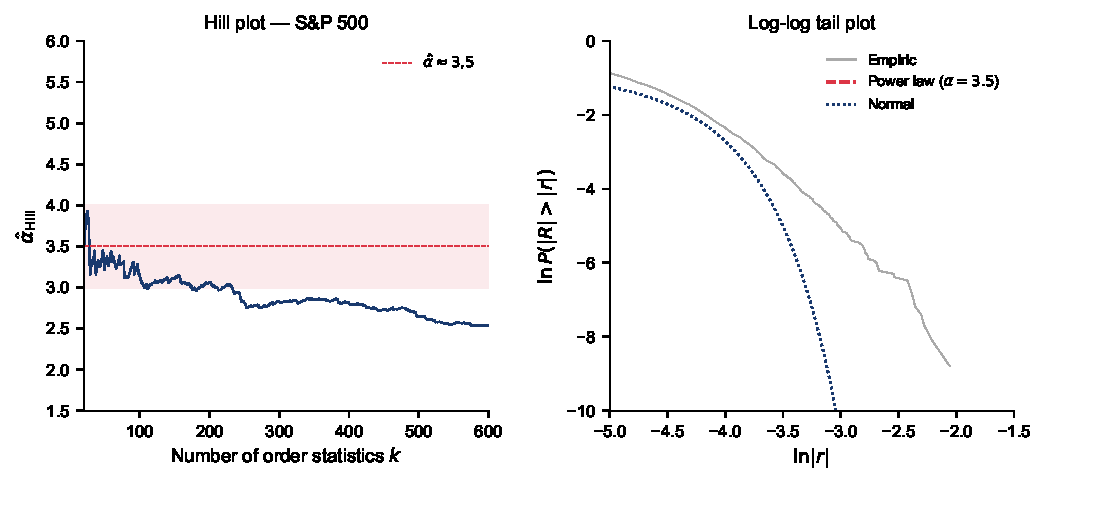
\includegraphics[width=\textwidth]{ch2_hill_plot.pdf}
            {\tiny Estimatorul Hill: $\hat{\alpha}$ pentru cozile Pareto}
        \end{column}
    \end{columns}
    \quantlet{SFM\_ch2\_extreme\_value}{https://github.com/QuantLet/Stat_fin_markets/tree/master/Ch_02/SFM_ch2_extreme_value}
\end{cminipage}
\end{frame}

\begin{frame}{Test 12: Teorema Limită Centrală}
\begin{cminipage}{0.95\textwidth}
    \begin{alertblock}{Întrebare}
        CLT garantează convergența mediei eșantionului la Normal. Care condiție este \textbf{esențială}?
    \end{alertblock}

    \vspace{0.5cm}
    \begin{block}{Variante de răspuns}
    \textcolor{MainBlue}{\textbf{(A)}} Distribuția originală trebuie să fie normală\\[3pt]
    \textcolor{MainBlue}{\textbf{(B)}} Varianța distribuției originale trebuie să fie finită\\[3pt]
    \textcolor{MainBlue}{\textbf{(C)}} Observațiile trebuie să fie corelate\\[3pt]
    \textcolor{MainBlue}{\textbf{(D)}} Eșantionul trebuie să fie mai mic de 30
    \end{block}
\end{cminipage}
\end{frame}

\begin{frame}{Test 12: Răspuns}
\begin{cminipage}{0.95\textwidth}
    \begin{columns}[T]
        \begin{column}{0.52\textwidth}
            \begin{exampleblock}{Răspuns: B}
                Varianță finită este condiția esențială
            \end{exampleblock}

            \vspace{0.2cm}

            \begin{itemize}\setlength{\itemsep}{0pt}
                \item \textbf{Teorema Limită Centrală (Lindeberg-Lévy):}
                \item Dacă $X_1, \ldots, X_n$ sunt i.i.d.\ cu $\E[X] = \mu$ și $\Var(X) = \sigma^2 < \infty$:
            \end{itemize}
            $$\frac{\bar{X}_n - \mu}{\sigma / \sqrt{n}} \xrightarrow{d} \mathcal{N}(0, 1)$$

            \begin{itemize}\setlength{\itemsep}{0pt}
                \item A: Distribuția originală poate fi \textit{orice} \incorrect
                \item B: $\sigma^2 < \infty$ este necesar \correct
                \item C: Observațiile trebuie să fie \textit{independente} \incorrect
                \item D: $n \to \infty$, nu $n < 30$ \incorrect
                \item \textbf{Fără} varianță finită $\Rightarrow$ convergență la distribuții \textit{stabile}
            \end{itemize}
        \end{column}
        \begin{column}{0.45\textwidth}
            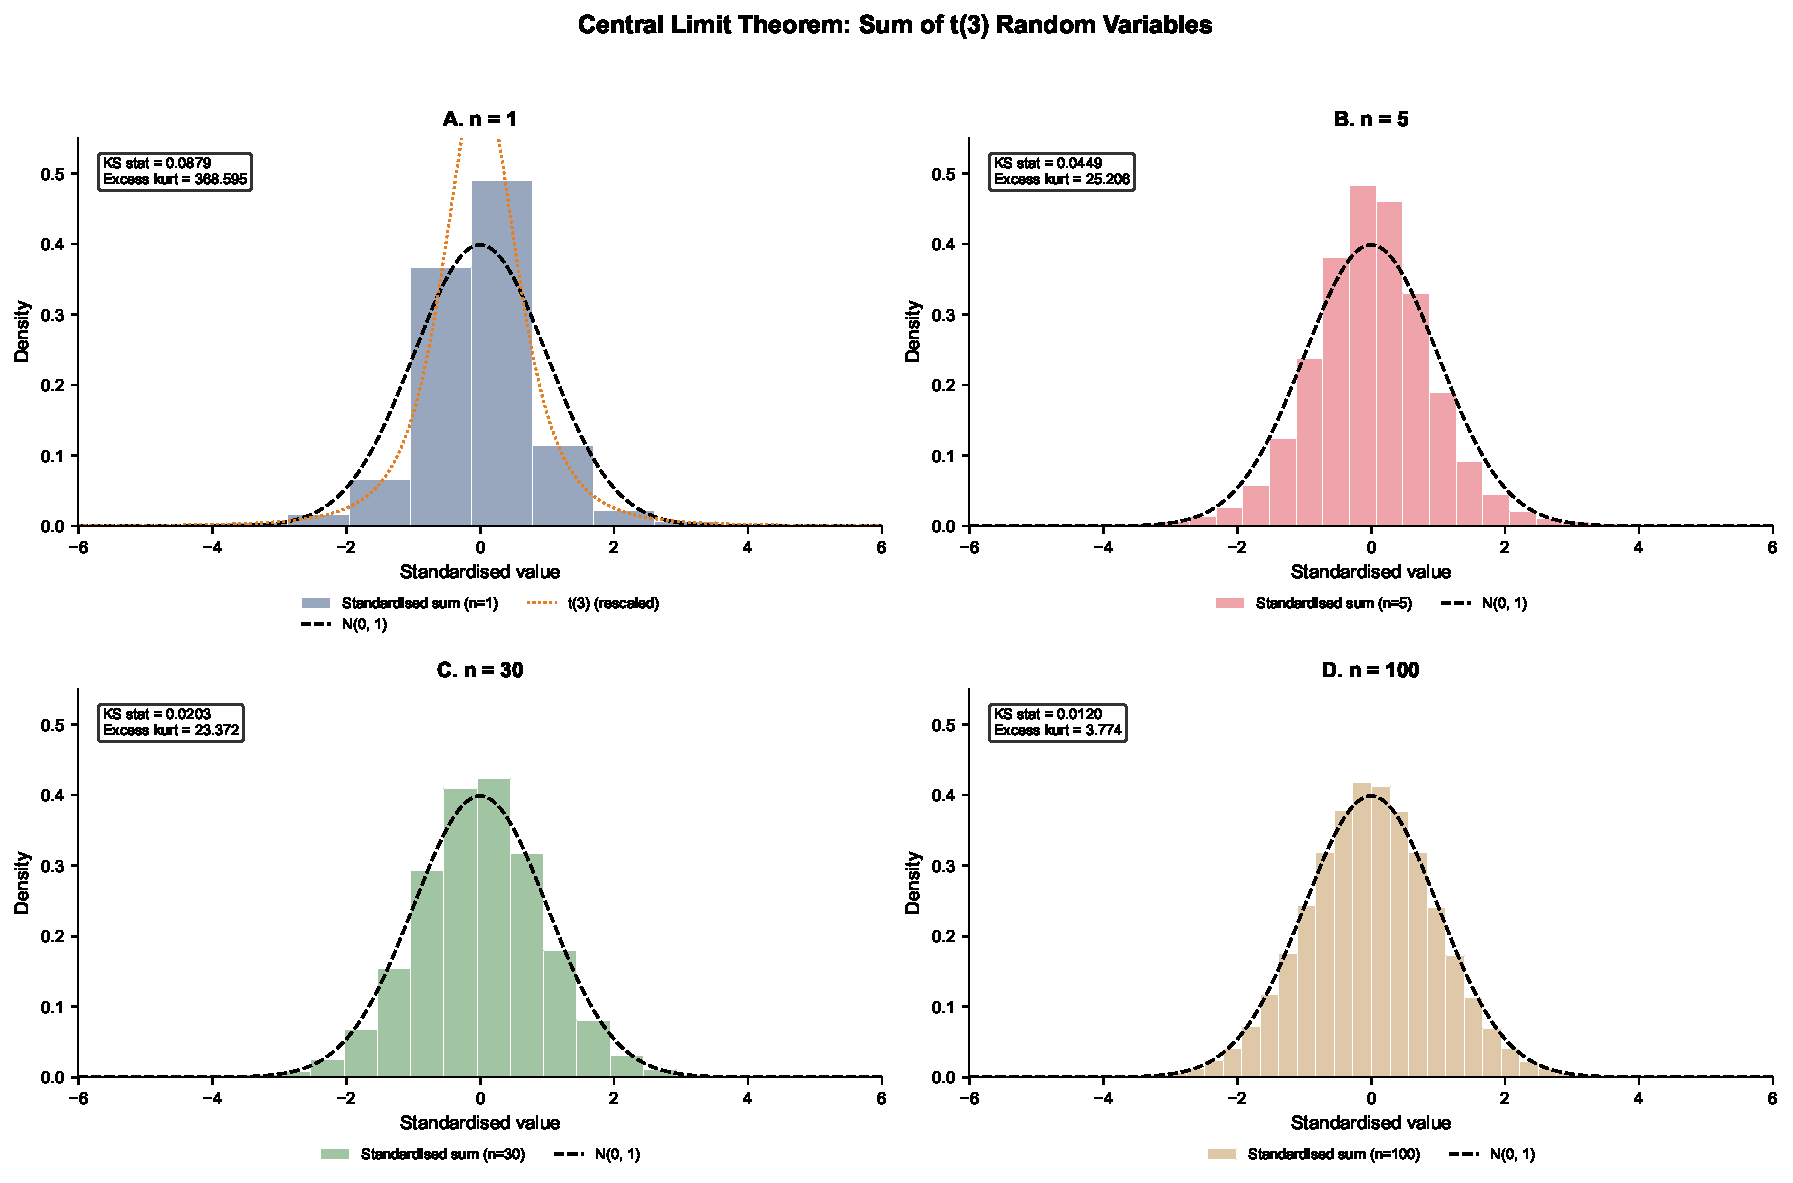
\includegraphics[width=\textwidth]{ch2_clt_illustration.pdf}
            {\tiny CLT: convergența la Normal pe măsură ce $n$ crește}
        \end{column}
    \end{columns}
\end{cminipage}
\end{frame}

\begin{frame}{Test 13: Interpretarea Q-Q Plot}
\begin{cminipage}{0.95\textwidth}
    \begin{alertblock}{Întrebare}
        Pe un Q-Q plot normal, punctele curbate \textbf{în sus} la capătul drept și \textbf{în jos} la capătul stâng indică:
    \end{alertblock}

    \vspace{0.5cm}
    \begin{block}{Variante de răspuns}
    \textcolor{MainBlue}{\textbf{(A)}} Normalitate perfectă\\[3pt]
    \textcolor{MainBlue}{\textbf{(B)}} Cozi mai ușoare decât normala\\[3pt]
    \textcolor{MainBlue}{\textbf{(C)}} Cozi mai grele decât normala\\[3pt]
    \textcolor{MainBlue}{\textbf{(D)}} Asimetrie pozitivă
    \end{block}
\end{cminipage}
\end{frame}

\begin{frame}{Test 13: Răspuns}
\begin{cminipage}{0.95\textwidth}
    \begin{columns}[T]
        \begin{column}{0.52\textwidth}
            \begin{exampleblock}{Răspuns: C}
                Cozi mai grele decât distribuția normală
            \end{exampleblock}

            \vspace{0.2cm}

            \begin{itemize}\setlength{\itemsep}{0pt}
                \item \textbf{Interpretarea Q-Q plot:}
                \item Linie dreaptă: distribuția se potrivește \correct
                \item Curbare în \textbf{S}: cozi grele (leptokurtosis)
                \item Capăt drept $\uparrow$: valori extreme pozitive mai mari
                \item Capăt stâng $\downarrow$: valori extreme negative mai mari
                \item $\Rightarrow$ Randamentele au mai multe \textbf{evenimente extreme} decât prezice distribuția normală
                \item Q-Q plot-ul este \textit{vizual}, nu un test formal
            \end{itemize}
        \end{column}
        \begin{column}{0.45\textwidth}
            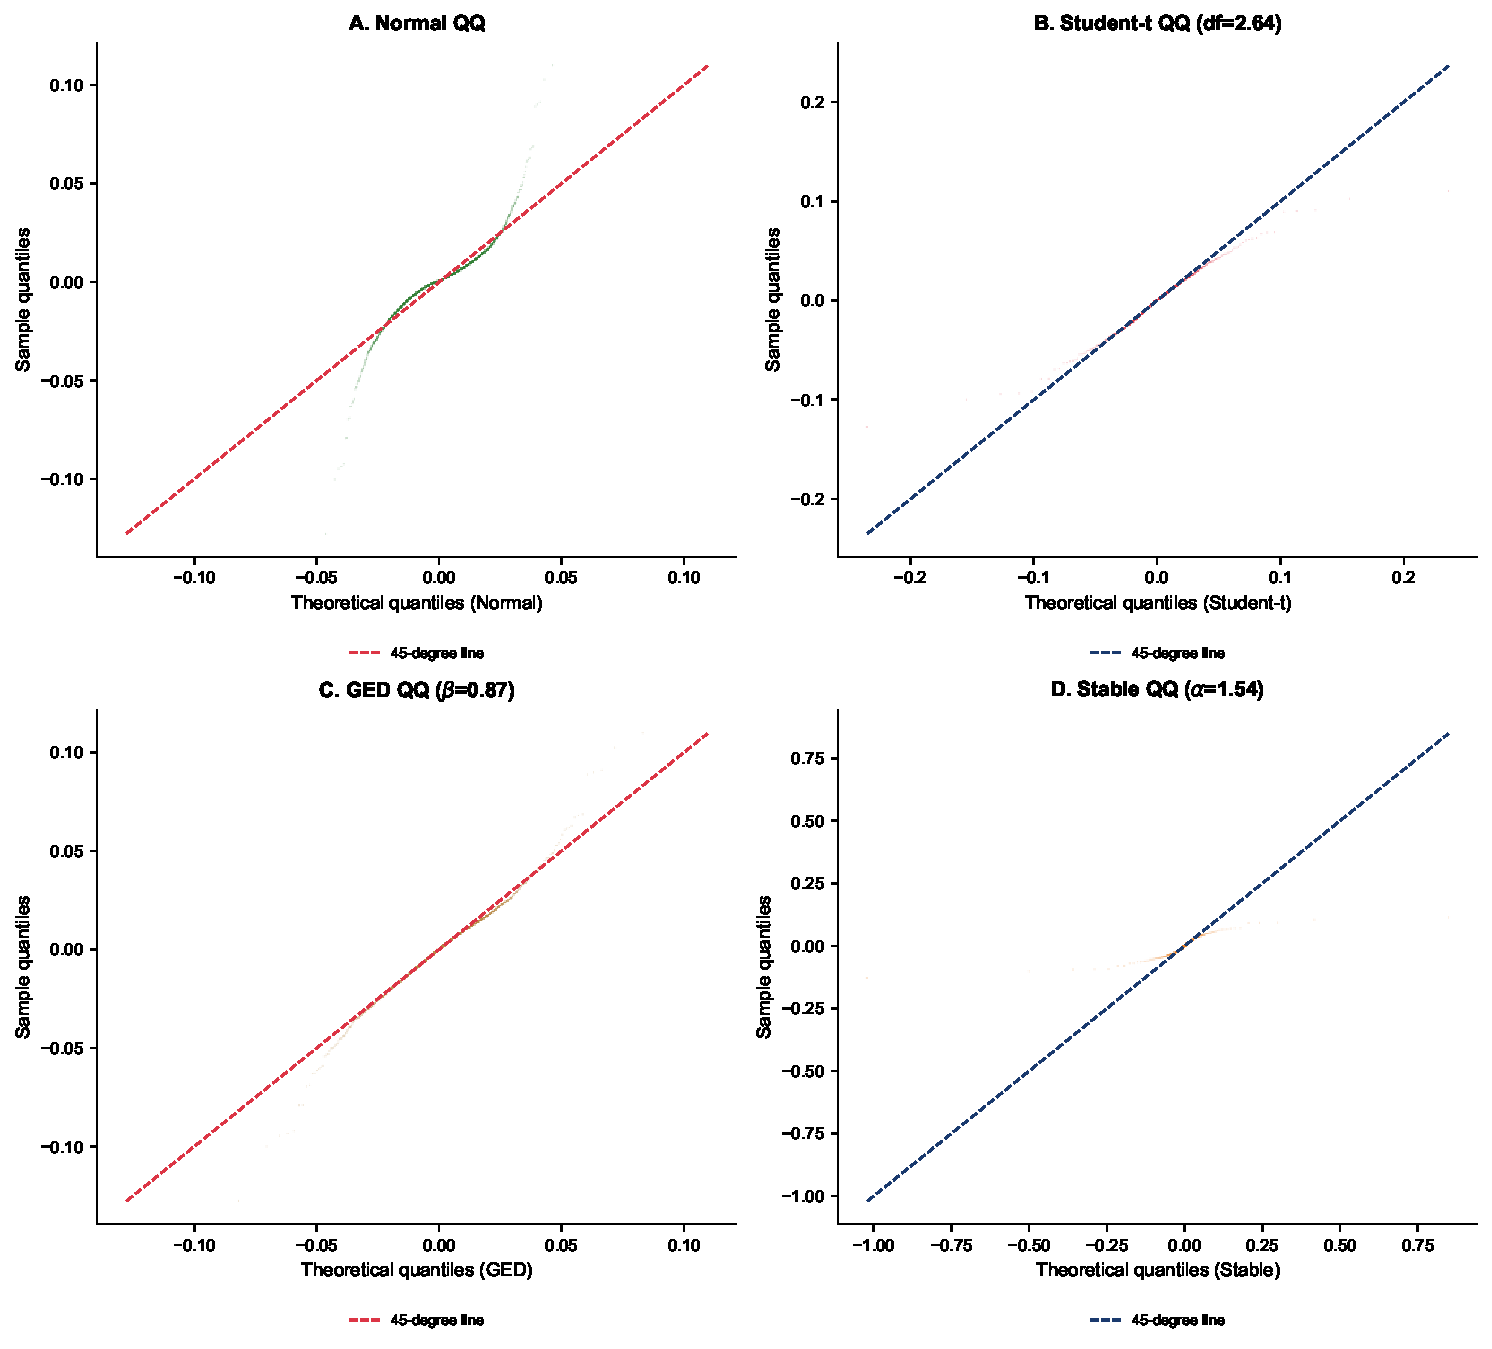
\includegraphics[width=\textwidth]{ch2_dist_comparison_qq.pdf}
            {\tiny Q-Q plot: deviațiile din cozi indică leptokurtosis}
        \end{column}
    \end{columns}
    \quantlet{SFM\_ch2\_distribution\_comparison}{https://github.com/QuantLet/Stat_fin_markets/tree/master/Ch_02/SFM_ch2_distribution_comparison}
\end{cminipage}
\end{frame}

\begin{frame}{Test 14: Subaditivitatea VaR}
\begin{cminipage}{0.95\textwidth}
    \begin{alertblock}{Întrebare}
        VaR nu este subaditivă. Ce înseamnă aceasta?
    \end{alertblock}

    \vspace{0.5cm}
    \begin{block}{Variante de răspuns}
    \textcolor{MainBlue}{\textbf{(A)}} $\text{VaR}(A+B) \leq \text{VaR}(A) + \text{VaR}(B)$ întotdeauna\\[3pt]
    \textcolor{MainBlue}{\textbf{(B)}} $\text{VaR}(A+B) > \text{VaR}(A) + \text{VaR}(B)$ este posibil\\[3pt]
    \textcolor{MainBlue}{\textbf{(C)}} VaR nu poate fi calculat pentru portofolii\\[3pt]
    \textcolor{MainBlue}{\textbf{(D)}} VaR este întotdeauna mai mare decât ES
    \end{block}
\end{cminipage}
\end{frame}

\begin{frame}{Test 14: Răspuns}
\begin{cminipage}{0.95\textwidth}
    \begin{columns}[T]
        \begin{column}{0.52\textwidth}
            \begin{exampleblock}{Răspuns: B}
                Diversificarea poate \textit{crește} VaR-ul
            \end{exampleblock}

            \vspace{0.2cm}

            \begin{itemize}\setlength{\itemsep}{0pt}
                \item \textbf{Lipsa subaditivității:}
                \item Există cazuri în care combinarea a 2 active \textbf{crește} VaR-ul total
                \item Aceasta contrazice principiul diversificării
                \item \textbf{Exemplu clasic:} două opțiuni digitale cu probabilități mici de pierdere
                \item ES satisface \textbf{întotdeauna} subaditivitatea:
            \end{itemize}
            $$\text{ES}(A+B) \leq \text{ES}(A) + \text{ES}(B)$$
            \begin{itemize}\setlength{\itemsep}{0pt}
                \item $\Rightarrow$ ES este o măsură de risc \textbf{coerentă}; VaR nu este
            \end{itemize}
        \end{column}
        \begin{column}{0.45\textwidth}
            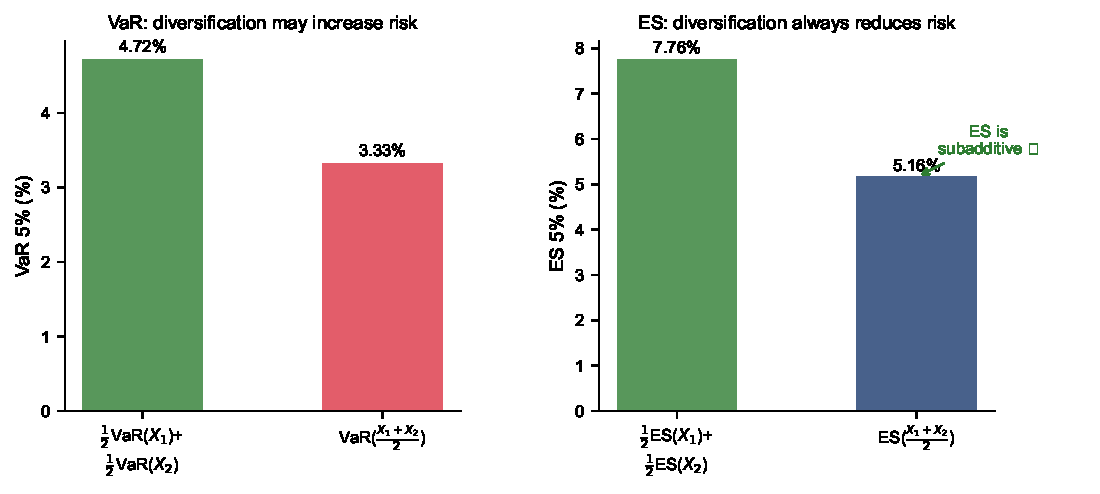
\includegraphics[width=\textwidth]{ch2_var_subadditivity.pdf}
            {\tiny VaR: diversificarea nu garantează reducerea}
        \end{column}
    \end{columns}
    \quantlet{SFM\_ch2\_risk\_management}{https://github.com/QuantLet/Stat_fin_markets/tree/master/Ch_02/SFM_ch2_risk_management}
\end{cminipage}
\end{frame}

\begin{frame}{Test 15: Momentele Distribuției Pareto}
\begin{cminipage}{0.95\textwidth}
    \begin{alertblock}{Întrebare}
        Dacă $X \sim \text{Pareto}(\alpha = 2.5)$, care momente sunt finite?
    \end{alertblock}

    \vspace{0.5cm}
    \begin{block}{Variante de răspuns}
    \textcolor{MainBlue}{\textbf{(A)}} Doar media\\[3pt]
    \textcolor{MainBlue}{\textbf{(B)}} Media și varianța\\[3pt]
    \textcolor{MainBlue}{\textbf{(C)}} Media, varianța și skewness\\[3pt]
    \textcolor{MainBlue}{\textbf{(D)}} Toate momentele
    \end{block}
\end{cminipage}
\end{frame}

\begin{frame}{Test 15: Răspuns}
\begin{cminipage}{0.95\textwidth}
    \begin{columns}[T]
        \begin{column}{0.52\textwidth}
            \begin{exampleblock}{Răspuns: B}
                Media și varianța, dar nu skewness
            \end{exampleblock}

            \vspace{0.2cm}

            \begin{itemize}\setlength{\itemsep}{0pt}
                \item \textbf{Regula momentelor Pareto:}
                \item $\E[X^p] < \infty$ dacă și numai dacă $p < \alpha$
                \item Cu $\alpha = 2.5$:
                \item $p = 1$ (media): $1 < 2.5$ \correct
                \item $p = 2$ (varianța): $2 < 2.5$ \correct
                \item $p = 3$ (skewness): $3 > 2.5$ \incorrect \ infinit
                \item \textbf{Ierarhia momentelor:}
            \end{itemize}
            \small
            \renewcommand{\arraystretch}{1.1}
            \begin{tabular}{ll}
            \toprule
            $\alpha > 1$ & Media finită \\
            $\alpha > 2$ & Varianța finită \\
            $\alpha > 3$ & Skewness finit \\
            $\alpha > 4$ & Kurtosis finită \\
            \bottomrule
            \end{tabular}
        \end{column}
        \begin{column}{0.45\textwidth}
            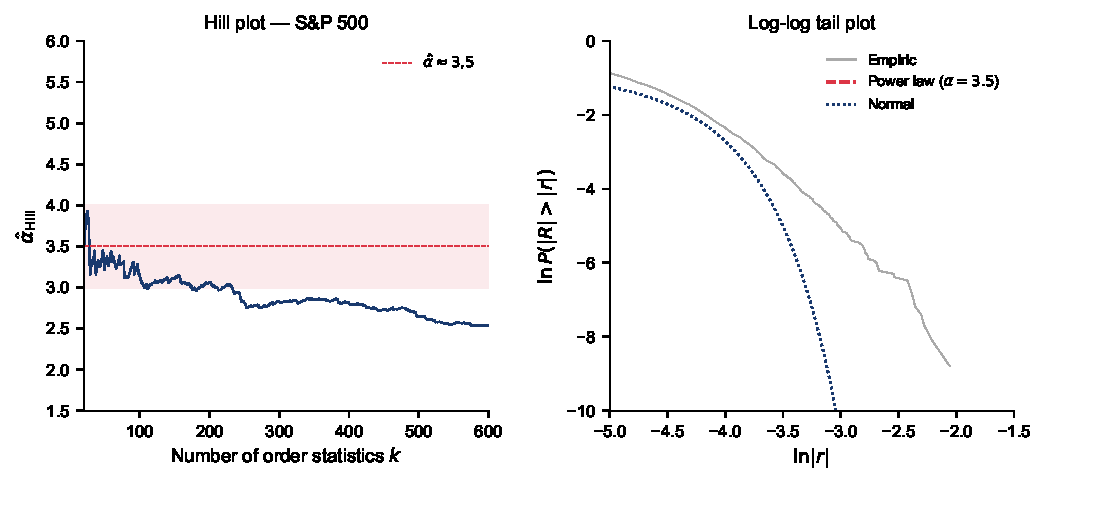
\includegraphics[width=\textwidth]{ch2_hill_plot.pdf}
            {\tiny Estimatorul Hill: $\hat{\alpha}$ determină ce momente există}
        \end{column}
    \end{columns}
    \quantlet{SFM\_ch2\_extreme\_value}{https://github.com/QuantLet/Stat_fin_markets/tree/master/Ch_02/SFM_ch2_extreme_value}
\end{cminipage}
\end{frame}

%=============================================================================
% PART 2: TRUE/FALSE QUESTIONS
%=============================================================================
\section{Întrebări Adevărat/Fals}

\begin{frame}{Adevărat sau Fals? --- Întrebări}
\begin{cminipage}{0.95\textwidth}
    \begin{itemize}\setlength{\itemsep}{0pt}
        \item \textbf{Răspundeți cu Adevărat (A) sau Fals (F):}
    \end{itemize}
    \vspace{0.3cm}
    \begin{enumerate}\setlength{\itemsep}{0pt}
        \item Distribuția normală este complet specificată de medie și varianță.
        \item Testul Jarque--Bera are putere mare pe eșantioane mici ($n < 30$).
        \item Excesul de kurtosis al distribuției Student-$t$ există pentru orice $\nu > 0$.
        \item VaR Normal subestimează riscul real la nivel de 1\% pe piețele financiare.
        \item ES este o măsură de risc coerentă, dar VaR nu este.
        \item AIC penalizează complexitatea mai mult decât BIC.
        \item Media distribuției Pareto cu $\alpha = 1.5$ este finită.
    \end{enumerate}
\end{cminipage}
\end{frame}

\begin{frame}{Adevărat sau Fals? --- Răspunsuri}
\begin{cminipage}{0.95\textwidth}
    \begin{columns}[T]
        \begin{column}{0.55\textwidth}
            \footnotesize
            \begin{enumerate}\setlength{\itemsep}{1pt}
                \item \textcolor{Forest}{\textbf{A}}: $\mathcal{N}(\mu, \sigma^2)$ are exact 2 parametri
                \item \textcolor{Crimson}{\textbf{F}}: JB are putere \textit{scăzută} pe eșantioane mici; necesită $n \geq 100$
                \item \textcolor{Crimson}{\textbf{F}}: Kurtosis există doar pentru $\nu > 4$; varianța doar pentru $\nu > 2$
                \item \textcolor{Forest}{\textbf{A}}: Cozile empirice sunt mai grele decât cele normale
                \item \textcolor{Forest}{\textbf{A}}: VaR nu este subaditivă; ES satisface axiomele de coerență
                \item \textcolor{Crimson}{\textbf{F}}: BIC penalizează \textit{mai mult} ($k\ln n$ vs $2k$ pentru $n > 7$)
                \item \textcolor{Forest}{\textbf{A}}: $\E[X] = \alpha x_m/(\alpha - 1)$ finită pentru $\alpha > 1$; cu $\alpha = 1.5$ $\Rightarrow$ media există
            \end{enumerate}
        \end{column}
        \begin{column}{0.42\textwidth}
            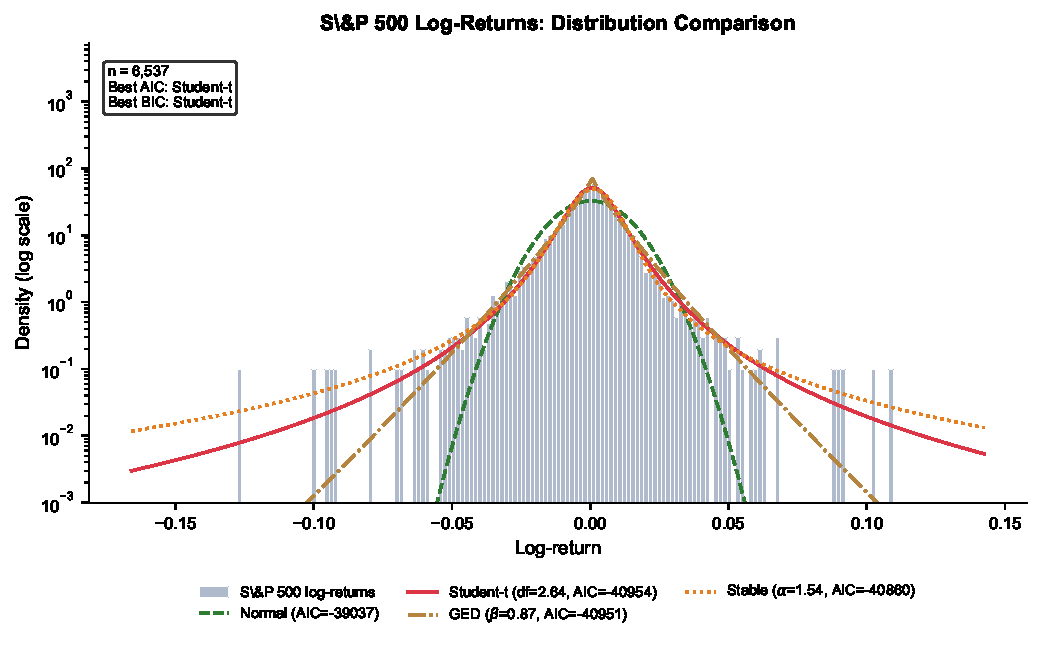
\includegraphics[width=\textwidth]{ch2_dist_comparison_overlay.pdf}
            {\tiny Normal vs Student-$t$ vs Empiric}
        \end{column}
    \end{columns}
    \quantlet{SFM\_ch2\_distribution\_comparison}{https://github.com/QuantLet/Stat_fin_markets/tree/master/Ch_02/SFM_ch2_distribution_comparison}
\end{cminipage}
\end{frame}

\begin{frame}{Adevărat sau Fals? --- Întrebări (Partea II)}
\begin{cminipage}{0.95\textwidth}
    \begin{itemize}\setlength{\itemsep}{0pt}
        \item \textbf{Răspundeți cu Adevărat (A) sau Fals (F):}
    \end{itemize}
    \vspace{0.3cm}
    \begin{enumerate}\setlength{\itemsep}{0pt}
        \setcounter{enumi}{7}
        \item Teorema Limită Centrală necesită varianță finită a distribuției originale.
        \item Q-Q plot-ul este un test \textit{formal} de normalitate (produce o $p$-valoare).
        \item Expected Shortfall este subaditivă pentru orice distribuție continuă.
        \item Distribuția Cauchy este Student-$t$ cu $\nu = 1$.
        \item Pareto cu $\alpha = 0.8$ are medie finită.
        \item VaR la 5\% este întotdeauna mai mare decât VaR la 1\%.
        \item Log-randamentele sunt preferate randamentelor simple deoarece sunt aditive în timp.
    \end{enumerate}
\end{cminipage}
\end{frame}

\begin{frame}{Adevărat sau Fals? --- Răspunsuri (Partea II)}
\begin{cminipage}{0.95\textwidth}
    \footnotesize
    \begin{enumerate}\setlength{\itemsep}{1pt}
        \setcounter{enumi}{7}
        \item \textcolor{Forest}{\textbf{A}}: CLT standard cere $\Var(X) < \infty$; fără varianță finită $\Rightarrow$ convergență către stabile, nu Normal
        \item \textcolor{Crimson}{\textbf{F}}: Q-Q plot-ul este un instrument \textit{grafic}, nu un test formal; testele formale sunt JB, SW, AD
        \item \textcolor{Forest}{\textbf{A}}: ES satisface subaditivitatea: $\text{ES}(A+B) \leq \text{ES}(A) + \text{ES}(B)$ --- proprietate cheie de coerență
        \item \textcolor{Forest}{\textbf{A}}: Cauchy $\equiv t_1$; nu are nici medie, nici varianță definite
        \item \textcolor{Crimson}{\textbf{F}}: Media Pareto există doar pentru $\alpha > 1$; cu $\alpha = 0.8 < 1$ $\Rightarrow$ medie infinită
        \item \textcolor{Crimson}{\textbf{F}}: VaR la 5\% $<$ VaR la 1\% (cuantila 5\% este mai aproape de centru decât cuantila 1\%)
        \item \textcolor{Forest}{\textbf{A}}: $r_{1 \to T} = \sum_{t=1}^T r_t$ --- aditivitate temporală; randamentele simple se compun multiplicativ
    \end{enumerate}
\end{cminipage}
\end{frame}

%=============================================================================
% PART 3: CALCULATION EXERCISES
%=============================================================================
\section{Exerciții de Calcul}

\begin{frame}{Exercițiul 1: Log-randamente și testul JB}
\begin{cminipage}{0.95\textwidth}
    \begin{itemize}\setlength{\itemsep}{0pt}
        \item \textbf{Problemă:} Prețurile de închidere pe 5 zile: $P_0 = 100$, $P_1 = 103$, $P_2 = 99$, $P_3 = 101$, $P_4 = 105$.
        \item Calculați:
    \end{itemize}
    \begin{enumerate}\setlength{\itemsep}{0pt}
        \item Log-randamentele $r_t = \ln(P_t / P_{t-1})$
        \item Media, varianța, skewness, kurtosis ale eșantionului
        \item Statistica Jarque--Bera și concluzia la 5\%
    \end{enumerate}
\end{cminipage}
\end{frame}

\begin{frame}{Exercițiul 1: Soluție}
\begin{cminipage}{0.95\textwidth}
    \begin{columns}[T]
        \begin{column}{0.52\textwidth}
            \begin{itemize}\setlength{\itemsep}{0pt}
                \item \textbf{1. Log-randamente:}
            \end{itemize}
            \small
            \renewcommand{\arraystretch}{1.1}
            \begin{tabular}{ccc}
            \toprule
            $t$ & $P_t/P_{t-1}$ & $r_t$ \\
            \midrule
            1 & 1.030 & 0.0296 \\
            2 & 0.961 & $-0.0396$ \\
            3 & 1.020 & 0.0200 \\
            4 & 1.040 & 0.0388 \\
            \bottomrule
            \end{tabular}
            \normalsize

            \vspace{0.2cm}
            \begin{itemize}\setlength{\itemsep}{0pt}
                \item \textbf{2. Momente:}
            $\bar{r} = 0.0122$, $s^2 = 0.001186$,
            $\hat{S} \approx -0.86$, $\hat{K} \approx 2.05$
                \item \textbf{3. JB:}
            $JB = \frac{4}{6}(0.74 + 0.23) = 0.64$
                \item $\chi^2_{0.05}(2) = 5.99 \Rightarrow$ \textcolor{Forest}{\textbf{Nu respingem}} $H_0$
                \item \textit{Atenție: putere scăzută cu $n=4$!}
            \end{itemize}
        \end{column}
        \begin{column}{0.45\textwidth}
            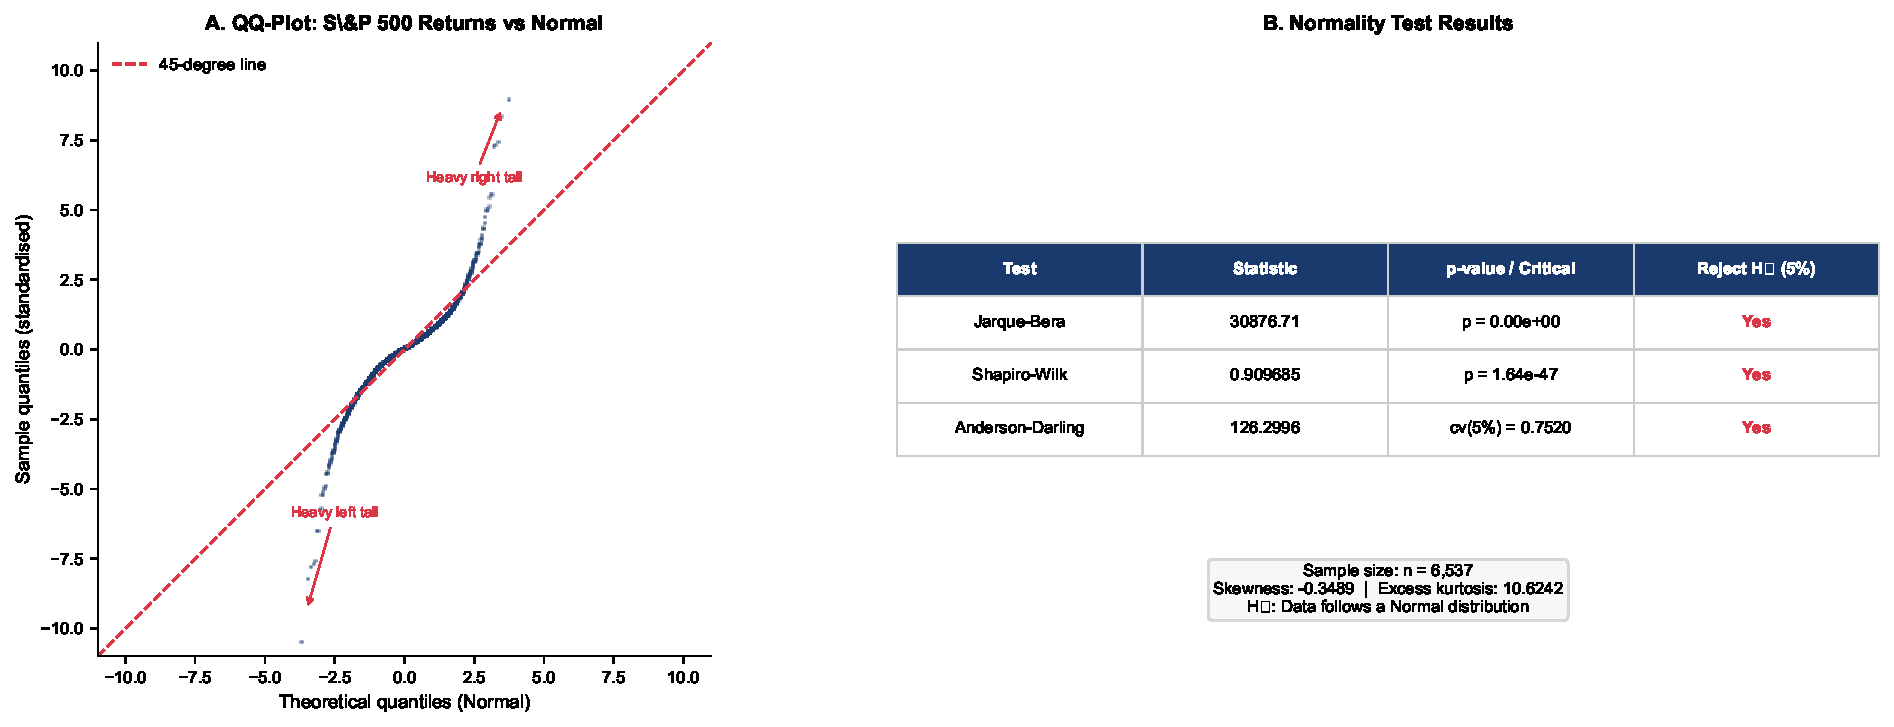
\includegraphics[width=\textwidth]{ch2_normality_tests.pdf}
            {\tiny Teste de normalitate pe randamente reale}
        \end{column}
    \end{columns}
    \quantlet{SFM\_ch2\_normal\_distribution}{https://github.com/QuantLet/Stat_fin_markets/tree/master/Ch_02/SFM_ch2_normal_distribution}
\end{cminipage}
\end{frame}

\begin{frame}{Exercițiul 2: VaR și ES Normal}
\begin{cminipage}{0.95\textwidth}
    \begin{itemize}\setlength{\itemsep}{0pt}
        \item \textbf{Problemă:} Portofoliu de 10\,000\,000 EUR, $\mu = 0.05\%$, $\sigma = 1.2\%$ zilnic.
        \item Calculați:
    \end{itemize}
    \begin{enumerate}\setlength{\itemsep}{0pt}
        \item VaR Normal la 5\%, 1\% și 0.1\%
        \item ES la 1\% sub ipoteza normală
        \item Raportul ES/VaR la 1\%
    \end{enumerate}
\end{cminipage}
\end{frame}

\begin{frame}{Exercițiul 2: Soluție}
\begin{cminipage}{0.95\textwidth}
    \begin{columns}[T]
        \begin{column}{0.52\textwidth}
            \begin{itemize}\setlength{\itemsep}{0pt}
                \item $\text{VaR}_\alpha = -(\mu + z_\alpha \sigma) \cdot W$
            \end{itemize}

            \vspace{0.2cm}
            \renewcommand{\arraystretch}{1.2}
            \begin{tabular}{ccc}
            \toprule
            $\alpha$ & $z_\alpha$ & \textbf{VaR (EUR)} \\
            \midrule
            5\% & $-1.645$ & 192\,400 \\
            1\% & $-2.326$ & 274\,100 \\
            0.1\% & $-3.090$ & 365\,800 \\
            \bottomrule
            \end{tabular}

            \vspace{0.2cm}
            \begin{itemize}\setlength{\itemsep}{0pt}
                \item \textbf{ES la 1\%:}
            \end{itemize}
            $$\text{ES}_{1\%} = -\mu + \sigma \frac{\phi(z_{0.01})}{0.01} = 3.13\%$$
            \begin{itemize}\setlength{\itemsep}{0pt}
                \item $\Rightarrow$ 313\,200 EUR
                \item \textbf{Raport:} $\text{ES}/\text{VaR} = 1.143$
            \end{itemize}
        \end{column}
        \begin{column}{0.45\textwidth}
            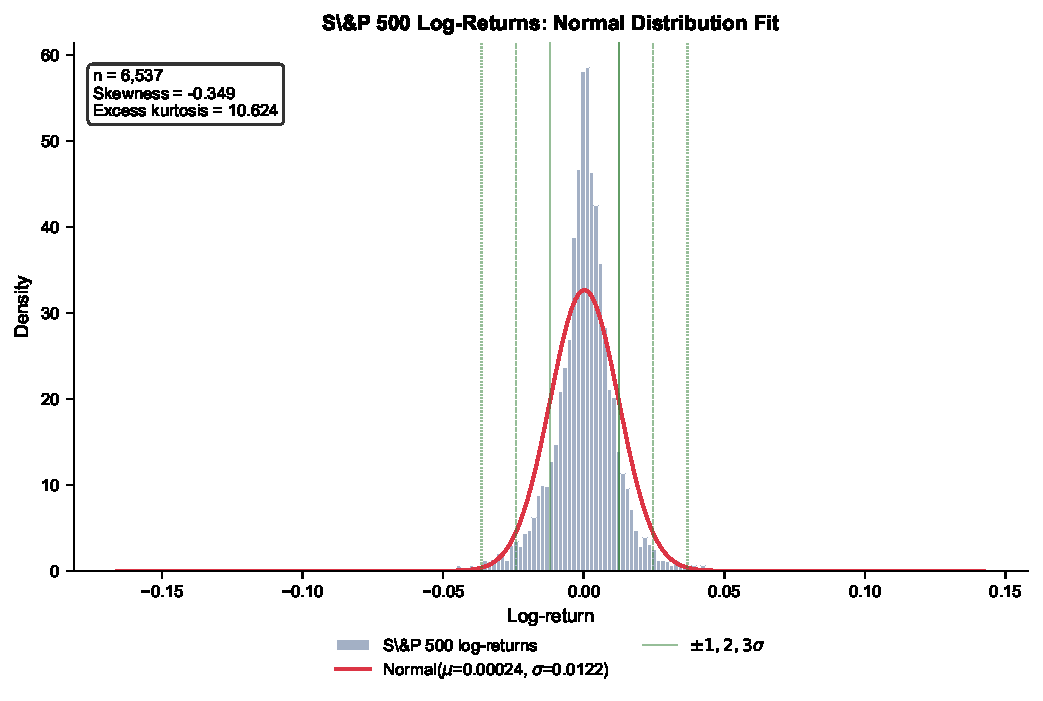
\includegraphics[width=\textwidth]{ch2_normal_fit.pdf}
            {\tiny VaR: cuantila din coada stângă}
        \end{column}
    \end{columns}
    \quantlet{SFM\_ch2\_risk\_management}{https://github.com/QuantLet/Stat_fin_markets/tree/master/Ch_02/SFM_ch2_risk_management}
\end{cminipage}
\end{frame}

\begin{frame}{Exercițiul 3: AIC/BIC --- Normal vs Student-$t$}
\begin{cminipage}{0.95\textwidth}
    \begin{itemize}\setlength{\itemsep}{0pt}
        \item \textbf{Problemă:} Pe $n = 2000$ randamente zilnice:
    \end{itemize}
    \begin{itemize}\setlength{\itemsep}{0pt}
        \item Normal ($k=2$): $\ell_N = 6421.3$
        \item Student-$t$ ($k=3$): $\ell_t = 6487.1$
    \end{itemize}
    \begin{itemize}\setlength{\itemsep}{0pt}
        \item Calculați AIC, BIC și interpretați.
    \end{itemize}
\end{cminipage}
\end{frame}

\begin{frame}{Exercițiul 3: Soluție}
\begin{cminipage}{0.95\textwidth}
    \begin{columns}[T]
        \begin{column}{0.52\textwidth}
            \begin{itemize}\setlength{\itemsep}{0pt}
                \item $\text{AIC} = -2\ell + 2k$, \quad $\text{BIC} = -2\ell + k\ln n$
            \end{itemize}

            \vspace{0.2cm}
            \renewcommand{\arraystretch}{1.3}
            \begin{tabular}{lccc}
            \toprule
            \textbf{Model} & $k$ & \textbf{AIC} & \textbf{BIC} \\
            \midrule
            Normal & 2 & $-12\,839$ & $-12\,827$ \\
            Student-$t$ & 3 & $-12\,968$ & $-12\,951$ \\
            \bottomrule
            \end{tabular}

            \vspace{0.2cm}
            \begin{itemize}\setlength{\itemsep}{0pt}
                \item $\Delta\text{AIC} = 129.6$
                \item $\Rightarrow$ Student-$t$ \textbf{foarte semnificativ} preferat ($\Delta > 10$)
                \item \textbf{Exces kurtosis:} $\kappa = 6/(\hat{\nu} - 4)$
                \item Cu $\hat{\nu} = 5.2$: $\kappa = 5.0$ (mult $> 0$)
            \end{itemize}
        \end{column}
        \begin{column}{0.45\textwidth}
            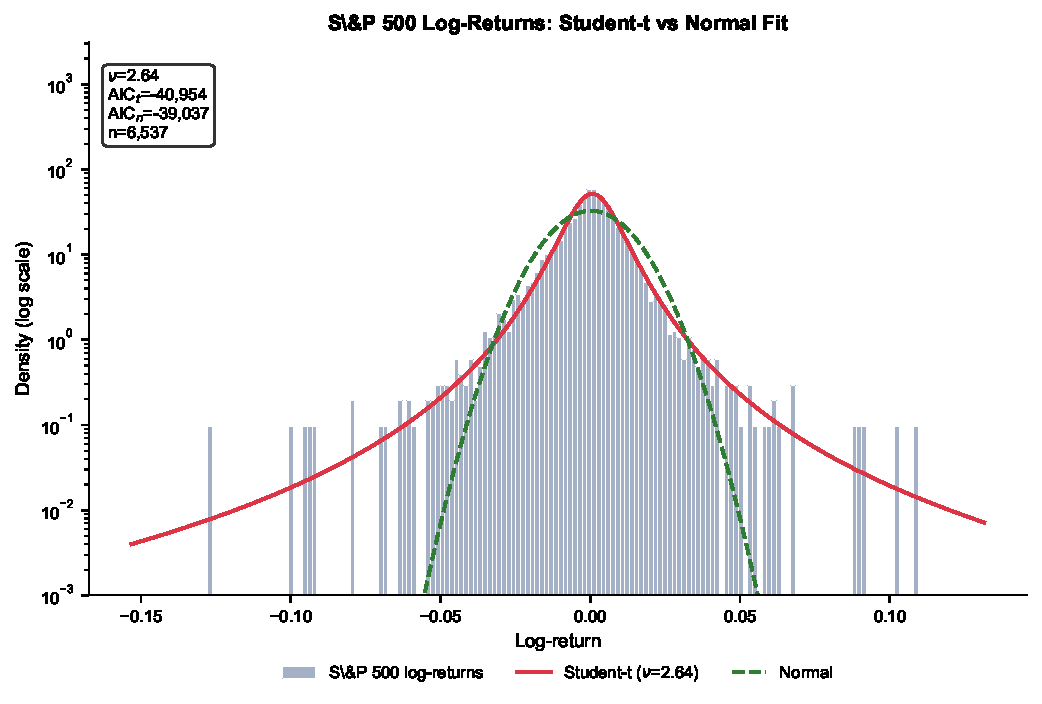
\includegraphics[width=\textwidth]{ch2_student_t_fit.pdf}
            {\tiny Student-$t$ fit: captează mai bine cozile}
        \end{column}
    \end{columns}
    \quantlet{SFM\_ch2\_student\_t}{https://github.com/QuantLet/Stat_fin_markets/tree/master/Ch_02/SFM_ch2_student_t}
\end{cminipage}
\end{frame}

\begin{frame}{Exercițiul 4: VaR Normal vs Student-$t$}
\begin{cminipage}{0.95\textwidth}
    \begin{itemize}\setlength{\itemsep}{0pt}
        \item \textbf{Problemă:} Portofoliu cu $\mu = 0$, $\sigma = 1.5\%$ zilnic. Student-$t$ cu $\hat{\nu} = 5$.
        \item Calculați:
    \end{itemize}
    \begin{enumerate}\setlength{\itemsep}{0pt}
        \item VaR la 1\% sub Normal și Student-$t$
        \item ES la 1\% sub ambele ipoteze
        \item Raportul ES/VaR pentru fiecare distribuție
    \end{enumerate}
\end{cminipage}
\end{frame}

\begin{frame}{Exercițiul 4: Soluție}
\begin{cminipage}{0.95\textwidth}
    \begin{columns}[T]
        \begin{column}{0.52\textwidth}
            \begin{itemize}\setlength{\itemsep}{0pt}
                \item $z_{1\%} = -2.326$, \; $t_{5}^{-1}(0.01) \approx -3.365$
                \item \textbf{1. VaR la 1\%:}
            \end{itemize}
            \renewcommand{\arraystretch}{1.2}
            \begin{tabular}{lc}
            \toprule
            \textbf{Model} & \textbf{VaR 1\%} \\
            \midrule
            Normal & $2.326 \times 1.5\% = \mathbf{3.49\%}$ \\
            Student-$t$ & $3.365 \times 1.5\% = \mathbf{5.05\%}$ \\
            \bottomrule
            \end{tabular}

            \vspace{0.2cm}
            \begin{itemize}\setlength{\itemsep}{0pt}
                \item \textbf{2. ES la 1\%:}
            \end{itemize}
            \begin{tabular}{lcc}
            \toprule
            & \textbf{ES} & \textbf{ES/VaR} \\
            \midrule
            Normal & 3.99\% & 1.14 \\
            Student-$t$ & 7.58\% & 1.50 \\
            \bottomrule
            \end{tabular}

            \begin{itemize}\setlength{\itemsep}{0pt}
                \item $\Rightarrow$ Student-$t$ dă VaR cu $\mathbf{45\%}$ mai mare.
            \end{itemize}
        \end{column}
        \begin{column}{0.45\textwidth}
            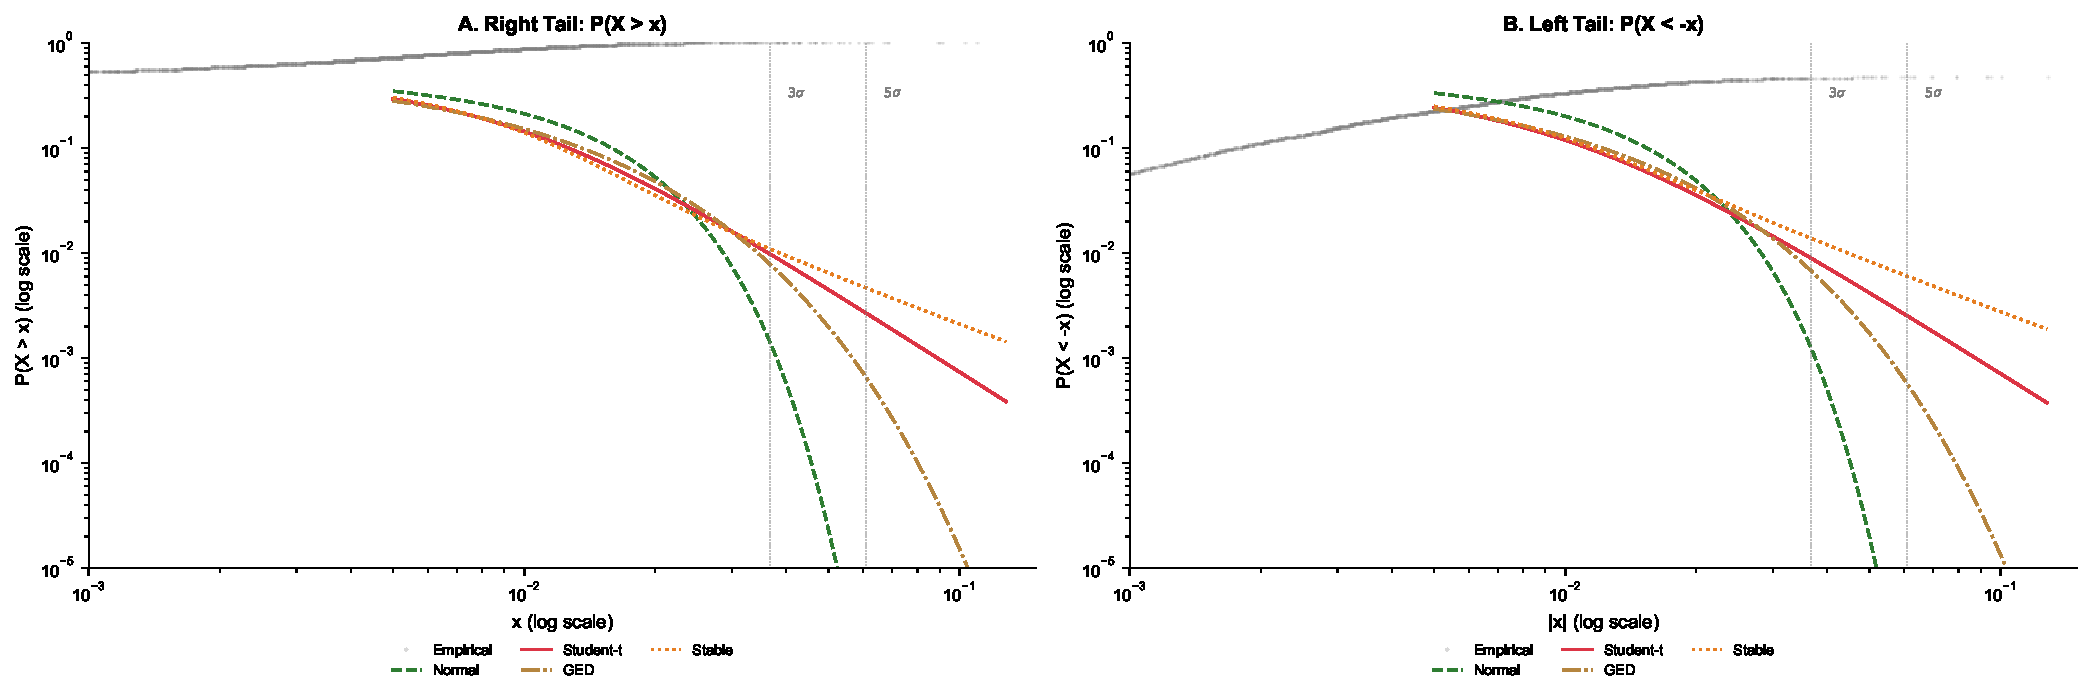
\includegraphics[width=\textwidth]{ch2_dist_comparison_tails.pdf}
            {\tiny Normal vs Student-$t$: diferența crește în cozi}
        \end{column}
    \end{columns}
    \quantlet{SFM\_ch2\_risk\_management}{https://github.com/QuantLet/Stat_fin_markets/tree/master/Ch_02/SFM_ch2_risk_management}
\end{cminipage}
\end{frame}

\begin{frame}{Exercițiul 5: Distribuția Pareto --- Cozi grele}
\begin{cminipage}{0.95\textwidth}
    \begin{itemize}\setlength{\itemsep}{0pt}
        \item \textbf{Problemă:} Pierderile extreme ale unui portofoliu urmează o distribuție Pareto cu $x_m = 2\%$ și $\alpha = 3$.
        \item Calculați:
    \end{itemize}
    \begin{enumerate}\setlength{\itemsep}{0pt}
        \item Probabilitatea unei pierderi mai mari de 4\%: $\Pr(X > 4\%)$
        \item Media pierderilor: $\E[X]$
        \item Varianța: $\Var(X)$
        \item VaR la 1\% (cuantila 99\%)
    \end{enumerate}
\end{cminipage}
\end{frame}

\begin{frame}{Exercițiul 5: Soluție}
\begin{cminipage}{0.95\textwidth}
    \small
    \vspace{-0.2cm}
    \begin{columns}[T]
        \begin{column}{0.55\textwidth}
            \begin{itemize}\setlength{\itemsep}{0pt}
                \item \textbf{1.} $\Pr(X > 4\%) = (x_m/x)^\alpha = (2/4)^3 = 1/8 = \mathbf{12.5\%}$
                \item \textbf{2.} Media ($\alpha = 3 > 1$):
            $\E[X] = \frac{\alpha x_m}{\alpha - 1} = \frac{3 \times 2\%}{2} = \mathbf{3\%}$
                \item \textbf{3.} Varianța ($\alpha = 3 > 2$):
            $\Var(X) = \frac{\alpha x_m^2}{(\alpha-1)^2(\alpha-2)} = \frac{12}{4} = \mathbf{3\%^2}$
                \item \textbf{4.} VaR la 1\%: $\Pr(X > q) = 0.01$
                \item $q = x_m (0.01)^{-1/\alpha} = 2\% \times 100^{1/3} \approx \mathbf{9.28\%}$
                \item VaR Pareto $= 9.28\%$ vs Normal $\approx 5.6\%$ ($+66\%$!)
            \end{itemize}
        \end{column}
        \begin{column}{0.42\textwidth}
            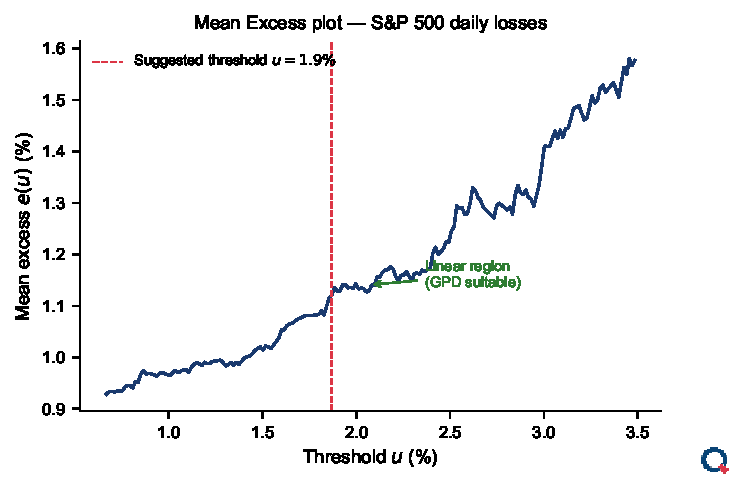
\includegraphics[width=\textwidth]{ch2_mean_excess_plot.pdf}
            {\tiny Mean excess plot: liniar $\Rightarrow$ coadă Pareto}
        \end{column}
    \end{columns}
    \quantlet{SFM\_ch2\_extreme\_value}{https://github.com/QuantLet/Stat_fin_markets/tree/master/Ch_02/SFM_ch2_extreme_value}
\end{cminipage}
\end{frame}

\begin{frame}{Exercițiul 6: Testul Raportului de Verosimilitate}
\begin{cminipage}{0.95\textwidth}
    \begin{itemize}\setlength{\itemsep}{0pt}
        \item \textbf{Problemă:} Pe $n = 1500$ randamente zilnice ale indicelui BET:
    \end{itemize}
    \begin{itemize}\setlength{\itemsep}{0pt}
        \item Normal ($k=2$): $\ell_N = 5102.7$
        \item Student-$t$ ($k=3$): $\ell_t = 5189.4$
    \end{itemize}
    \begin{enumerate}\setlength{\itemsep}{0pt}
        \item Calculați statistica testului raportului de verosimilitate (LR)
        \item Testul este la nivel de semnificație $\alpha = 1\%$. Respingem $H_0$: Normal?
        \item Estimați $\hat{\nu}$ din relația $\hat{\kappa} = 4.8$ (exces kurtosis eșantion)
    \end{enumerate}
\end{cminipage}
\end{frame}

\begin{frame}{Exercițiul 6: Soluție}
\begin{cminipage}{0.95\textwidth}
    \begin{columns}[T]
        \begin{column}{0.52\textwidth}
            \begin{itemize}\setlength{\itemsep}{0pt}
                \item \textbf{1. Statistica LR:}
            \end{itemize}
            $$LR = 2(\ell_t - \ell_N) = 2(5189.4 - 5102.7) = \mathbf{173.4}$$

            \begin{itemize}\setlength{\itemsep}{0pt}
                \item \textbf{2. Test:} $LR \sim \chi^2(1)$ sub $H_0$
                \item $\chi^2_{0.01}(1) = 6.635$
                \item $173.4 \gg 6.635$ $\Rightarrow$ \textcolor{Crimson}{\textbf{Respingem}} $H_0$
                \item $p$-value $\approx 0$ --- normalitatea este clar respinsă
                \item \textbf{3. Estimare $\hat{\nu}$:}
                \item $\kappa = 6/(\nu - 4) = 4.8$
                \item $\nu - 4 = 6/4.8 = 1.25$
                \item $\hat{\nu} = \mathbf{5.25}$ (tipic pentru acțiuni)
            \end{itemize}
        \end{column}
        \begin{column}{0.45\textwidth}
            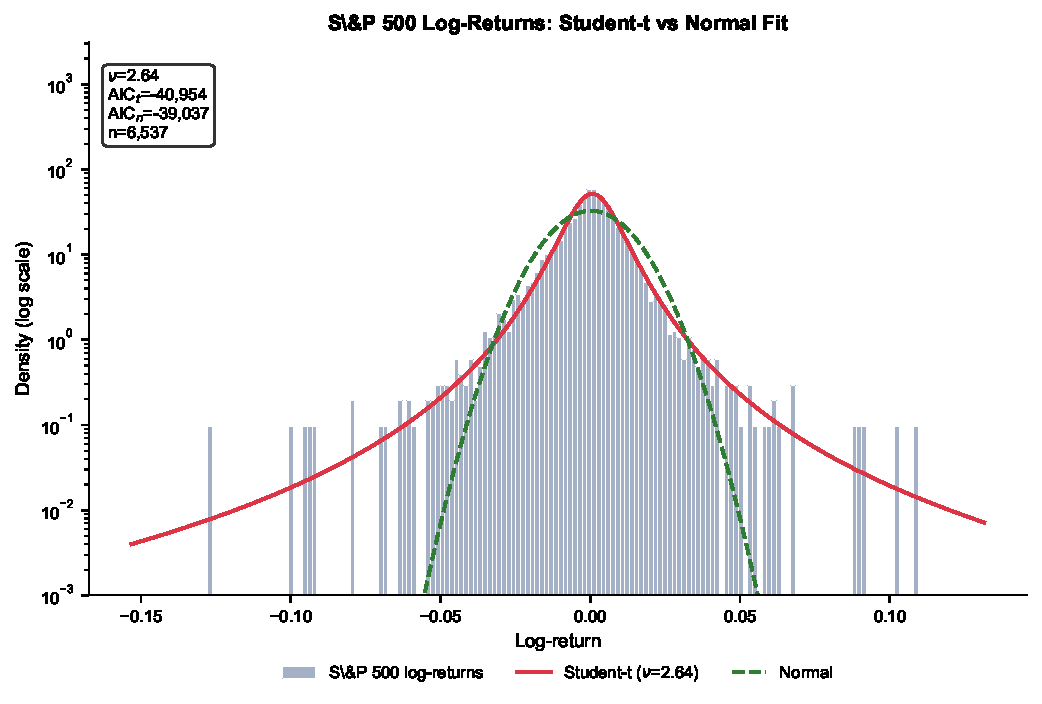
\includegraphics[width=\textwidth]{ch2_student_t_fit.pdf}
            {\tiny LR test: Student-$t$ semnificativ mai bun}
        \end{column}
    \end{columns}
    \quantlet{SFM\_ch2\_student\_t}{https://github.com/QuantLet/Stat_fin_markets/tree/master/Ch_02/SFM_ch2_student_t}
\end{cminipage}
\end{frame}

\begin{frame}{Exercițiul 7: Comparație Cross-Asset --- VaR și ES}
\begin{cminipage}{0.95\textwidth}
    \begin{itemize}\setlength{\itemsep}{0pt}
        \item \textbf{Problemă:} Trei active cu randamente zilnice estimate:
    \end{itemize}
    \vspace{0.1cm}
    \small
    \renewcommand{\arraystretch}{1.2}
    \begin{tabular}{lccccc}
    \toprule
    \textbf{Activ} & $\hat{\mu}$ & $\hat{\sigma}$ & $\hat{\nu}$ & $\hat{S}$ & $\hat{K}$ \\
    \midrule
    S\&P 500 & 0.04\% & 1.1\% & 5.2 & $-0.3$ & 5.5 \\
    Bitcoin & 0.10\% & 3.8\% & 3.5 & $-0.1$ & 8.0 \\
    Obligațiuni (10Y) & 0.01\% & 0.4\% & 7.8 & 0.1 & 3.8 \\
    \bottomrule
    \end{tabular}
    \normalsize
    \vspace{0.1cm}
    \begin{enumerate}\setlength{\itemsep}{0pt}
        \item Calculați VaR Normal la 1\% pentru fiecare activ
        \item Calculați VaR Student-$t$ la 1\% (folosind tabelul cuantilelor)
        \item Pentru care activ diferența Normal vs Student-$t$ este cea mai mare?
    \end{enumerate}
\end{cminipage}
\end{frame}

\begin{frame}{Exercițiul 7: Soluție}
\begin{cminipage}{0.95\textwidth}
    \small
    \begin{columns}[T]
        \begin{column}{0.55\textwidth}
            \begin{itemize}\setlength{\itemsep}{0pt}
                \item \textbf{Cuantile cheie:} $z_{1\%} = 2.326$
                \item $t_{5.2}^{-1}(0.01) \approx 3.30$, $t_{3.5}^{-1}(0.01) \approx 4.14$, $t_{7.8}^{-1}(0.01) \approx 2.78$
            \end{itemize}

            \vspace{0.1cm}
            \renewcommand{\arraystretch}{1.2}
            \begin{tabular}{lccc}
            \toprule
            \textbf{Activ} & \textbf{VaR$_N$} & \textbf{VaR$_t$} & \textbf{$\Delta$\%} \\
            \midrule
            S\&P 500 & 2.52\% & 3.59\% & +42\% \\
            Bitcoin & 8.74\% & 15.63\% & \textcolor{Crimson}{\textbf{+79\%}} \\
            Oblig.\ 10Y & 0.92\% & 1.10\% & +20\% \\
            \bottomrule
            \end{tabular}

            \vspace{0.15cm}
            \begin{itemize}\setlength{\itemsep}{0pt}
                \item $\Rightarrow$ \textbf{Bitcoin}: cel mai mare impact al cozilor
                \item Motiv: $\hat{\nu} = 3.5$ (kurtosis foarte ridicată)
                \item Obligațiunile: aproape de Normal ($\hat{\nu} = 7.8$)
            \end{itemize}
        \end{column}
        \begin{column}{0.42\textwidth}
            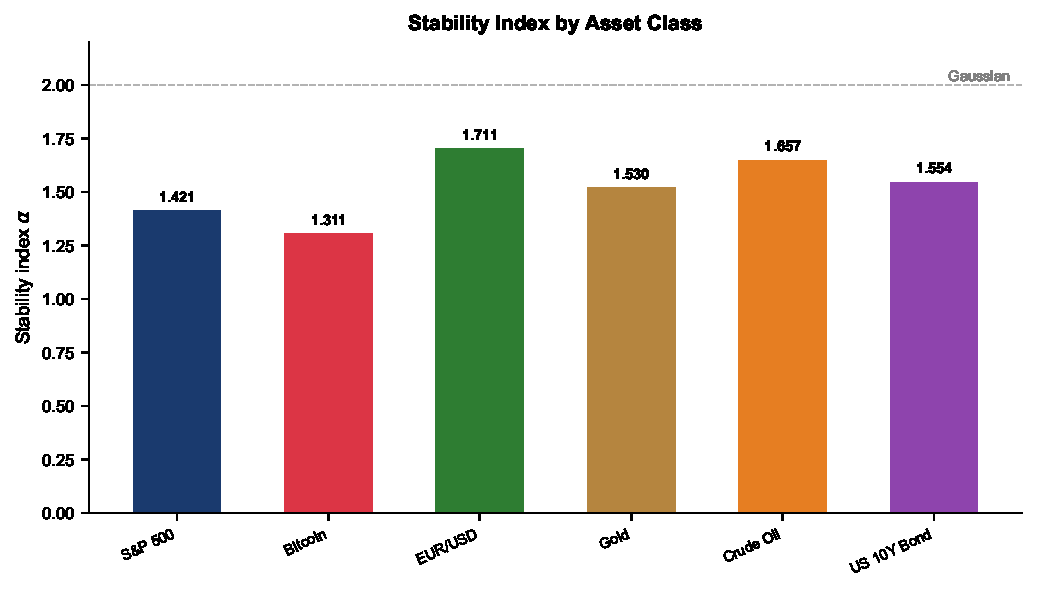
\includegraphics[width=\textwidth]{ch2_cross_asset_alpha.pdf}
            {\tiny Cross-asset: estimări $\hat{\alpha}$ diferite}
        \end{column}
    \end{columns}
    \quantlet{SFM\_ch2\_case\_study\_2a}{https://github.com/QuantLet/Stat_fin_markets/tree/master/Ch_02/SFM_ch2_case_study_2a}
\end{cminipage}
\end{frame}

\begin{frame}{Exercițiul 8: Funcția Mean Excess și Coadă Pareto}
\begin{cminipage}{0.95\textwidth}
    \begin{itemize}\setlength{\itemsep}{0pt}
        \item \textbf{Problemă:} Pierderile peste pragul $u$ au funcția mean excess $e(u) = \E[X - u \mid X > u]$.
        \item Pentru Pareto($x_m, \alpha$): $e(u) = u / (\alpha - 1)$.
        \item Datele: pentru praguri $u = 2\%, 3\%, 4\%, 5\%$, media excesurilor observate este:
    \end{itemize}
    \renewcommand{\arraystretch}{1.1}
    \begin{tabular}{ccccc}
    \toprule
    $u$ & 2\% & 3\% & 4\% & 5\% \\
    \midrule
    $\hat{e}(u)$ & 1.05\% & 1.48\% & 2.10\% & 2.45\% \\
    \bottomrule
    \end{tabular}
    \begin{enumerate}\setlength{\itemsep}{0pt}
        \item Verificați dacă $\hat{e}(u)$ este aproximativ liniară în $u$ (justifică Pareto?)
        \item Estimați $\hat{\alpha}$ din panta relației $e(u) = u/(\alpha-1)$
        \item Calculați VaR la 1\% folosind $\hat{\alpha}$ estimat și $x_m = 2\%$
    \end{enumerate}
\end{cminipage}
\end{frame}

\begin{frame}{Exercițiul 8: Soluție}
\begin{cminipage}{0.95\textwidth}
    \begin{columns}[T]
        \begin{column}{0.55\textwidth}
            \begin{itemize}\setlength{\itemsep}{0pt}
                \item \textbf{1. Liniaritate:} raportul $\hat{e}(u)/u$:
            \end{itemize}
            \small
            \renewcommand{\arraystretch}{1.1}
            \begin{tabular}{ccc}
            \toprule
            $u$ & $\hat{e}(u)$ & $\hat{e}(u)/u$ \\
            \midrule
            2\% & 1.05\% & 0.525 \\
            3\% & 1.48\% & 0.493 \\
            4\% & 2.10\% & 0.525 \\
            5\% & 2.45\% & 0.490 \\
            \bottomrule
            \end{tabular}
            \normalsize

            \begin{itemize}\setlength{\itemsep}{0pt}
                \item Raport $\approx 0.51$ (liniar) $\Rightarrow$ \textcolor{Forest}{\textbf{Pareto justificat}}
                \item \textbf{2.} $1/(\alpha-1) \approx 0.51 \Rightarrow \hat{\alpha} \approx \mathbf{2.96}$
                \item \textbf{3. VaR 1\%:}
                \item $q = x_m \cdot (0.01)^{-1/\alpha} = 2\% \times 100^{1/2.96}$
                \item $= 2\% \times 4.73 \approx \mathbf{9.46\%}$
            \end{itemize}
        \end{column}
        \begin{column}{0.42\textwidth}
            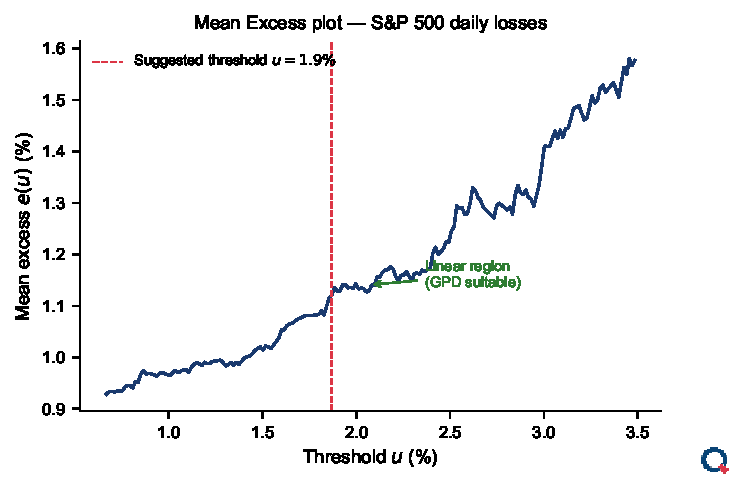
\includegraphics[width=\textwidth]{ch2_mean_excess_plot.pdf}
            {\tiny Mean excess liniar $\Rightarrow$ coadă Pareto}
        \end{column}
    \end{columns}
    \quantlet{SFM\_ch2\_extreme\_value}{https://github.com/QuantLet/Stat_fin_markets/tree/master/Ch_02/SFM_ch2_extreme_value}
\end{cminipage}
\end{frame}

%=============================================================================
% PART 4: PYTHON EXERCISES
%=============================================================================
\section{Exerciții Python}

\begin{frame}[fragile]{Exercițiu Python 1: Descărcare și teste de normalitate}
    \textbf{Sarcină:}
    \begin{enumerate}\setlength{\itemsep}{0pt}
        \item Descărcați datele S\&P 500 din ultimii 5 ani cu \texttt{yfinance}
        \item Calculați statisticile descriptive (medie, std, skewness, kurtosis)
        \item Aplicați testul Jarque--Bera și Shapiro--Wilk
    \end{enumerate}

    \vspace{0.3cm}
    \textbf{Cod cheie:}
    \begin{verbatim}
import yfinance as yf
from scipy import stats
data = yf.download('^GSPC', start='2020-01-01', end='2025-01-01')
returns = np.log(data['Adj Close'] / data['Adj Close'].shift(1)).dropna()
jb_stat, jb_pval = stats.jarque_bera(returns)
    \end{verbatim}

    \quantlet{SFM\_ch2\_normal\_distribution}{https://github.com/QuantLet/Stat_fin_markets/tree/master/Ch_02/SFM_ch2_normal_distribution}
\end{frame}

\begin{frame}[fragile]{Exercițiu Python 2: Estimare MLE și AIC/BIC}
    \textbf{Sarcină:}
    \begin{enumerate}\setlength{\itemsep}{0pt}
        \item Ajustați Normal și Student-$t$ prin MLE
        \item Calculați AIC și BIC pentru fiecare model
        \item Comparați și selectați cel mai bun model
    \end{enumerate}

    \vspace{0.3cm}
    \textbf{Cod cheie:}
    \begin{verbatim}
mu_n, sigma_n = stats.norm.fit(returns)
df_t, loc_t, sc_t = stats.t.fit(returns)
ll_n = np.sum(stats.norm.logpdf(returns, mu_n, sigma_n))
ll_t = np.sum(stats.t.logpdf(returns, df_t, loc_t, sc_t))
aic_n = -2*ll_n + 2*2;  aic_t = -2*ll_t + 2*3
    \end{verbatim}

    \quantlet{SFM\_ch2\_student\_t}{https://github.com/QuantLet/Stat_fin_markets/tree/master/Ch_02/SFM_ch2_student_t}
\end{frame}

\begin{frame}[fragile]{Exercițiu Python 3: Comparație VaR}
    \textbf{Sarcină:}
    \begin{enumerate}\setlength{\itemsep}{0pt}
        \item Calculați VaR la 5\%, 1\%, 0.1\% sub Normal, Student-$t$ și Empiric
        \item Vizualizați histograma cu overlay Normal vs Student-$t$ (log-scale)
        \item Calculați ES prin Monte Carlo sub Student-$t$
    \end{enumerate}

    \vspace{0.3cm}
    \textbf{Funcții cheie:}
    \begin{itemize}\setlength{\itemsep}{0pt}
        \item \texttt{stats.norm.ppf(alpha)} pentru cuantila normală
        \item \texttt{stats.t.ppf(alpha, df)} pentru cuantila Student-$t$
        \item \texttt{np.quantile(returns, alpha)} pentru cuantila empirică
    \end{itemize}

    \quantlet{SFM\_ch2\_distribution\_comparison}{https://github.com/QuantLet/Stat_fin_markets/tree/master/Ch_02/SFM_ch2_distribution_comparison}
\end{frame}

\begin{frame}[fragile]{Exercițiu Python 4: Pareto --- Fit și VaR}
    \textbf{Sarcină:}
    \begin{enumerate}\setlength{\itemsep}{0pt}
        \item Extrageți pierderile extreme (peste cuantila 95\%) din S\&P 500
        \item Ajustați o distribuție Pareto pe aceste pierderi
        \item Comparați VaR Pareto vs VaR Normal la 1\% și 0.1\%
    \end{enumerate}

    \vspace{0.3cm}
    \textbf{Cod cheie:}
    \begin{verbatim}
losses = -returns[returns < 0]
threshold = np.quantile(losses, 0.95)
tail = losses[losses > threshold]
alpha_hat, loc, scale = stats.pareto.fit(tail, floc=0)
var_pareto = stats.pareto.ppf(0.99, alpha_hat, loc, scale)
    \end{verbatim}

    \quantlet{SFM\_ch2\_extreme\_value}{https://github.com/QuantLet/Stat_fin_markets/tree/master/Ch_02/SFM_ch2_extreme_value}
\end{frame}

\begin{frame}[fragile]{Exercițiu Python 5: Q-Q Plots și Diagnostice Vizuale}
    \textbf{Sarcină:}
    \begin{enumerate}\setlength{\itemsep}{0pt}
        \item Construiți Q-Q plot-uri ale randamentelor S\&P 500 față de Normal și Student-$t$
        \item Adăugați intervalul de încredere 95\% pe Q-Q plot
        \item Interpretați abaterile din cozi
    \end{enumerate}

    \vspace{0.3cm}
    \textbf{Cod cheie:}
    \begin{verbatim}
from scipy import stats
import matplotlib.pyplot as plt
# Q-Q plot Normal
stats.probplot(returns, dist="norm", plot=plt)
# Q-Q plot Student-t
df_hat = stats.t.fit(returns)[0]
stats.probplot(returns, dist=stats.t, sparams=(df_hat,), plot=plt)
    \end{verbatim}

    \quantlet{SFM\_ch2\_distribution\_comparison}{https://github.com/QuantLet/Stat_fin_markets/tree/master/Ch_02/SFM_ch2_distribution_comparison}
\end{frame}

\begin{frame}[fragile]{Exercițiu Python 6: Bootstrap VaR și Intervale de Încredere}
    \textbf{Sarcină:}
    \begin{enumerate}\setlength{\itemsep}{0pt}
        \item Estimați VaR la 1\% prin bootstrap (10\,000 re-eșantionări)
        \item Calculați intervalul de încredere 95\% pentru VaR
        \item Comparați VaR bootstrap cu VaR parametric (Normal, Student-$t$)
    \end{enumerate}

    \vspace{0.3cm}
    \textbf{Cod cheie:}
    \begin{verbatim}
n_boot = 10000
var_boot = np.zeros(n_boot)
for i in range(n_boot):
    sample = np.random.choice(returns, size=len(returns), replace=True)
    var_boot[i] = -np.quantile(sample, 0.01)
ci_lower, ci_upper = np.quantile(var_boot, [0.025, 0.975])
    \end{verbatim}

    \quantlet{SFM\_ch2\_risk\_management}{https://github.com/QuantLet/Stat_fin_markets/tree/master/Ch_02/SFM_ch2_risk_management}
\end{frame}

%=============================================================================
% PART 5: DISCUSSION QUESTIONS
%=============================================================================
\section{Întrebări de Discuție}

\begin{frame}{Discuție 1: Normalitatea pe piețele financiare}
\begin{cminipage}{0.95\textwidth}
    \begin{itemize}\setlength{\itemsep}{0pt}
        \item \textbf{Scenariu:} Testul JB respinge normalitatea pe S\&P 500 ($p < 0.001$), dar managementul riscului folosește încă VaR Normal.
        \item \textbf{Întrebări:}
    \end{itemize}
    \begin{enumerate}\setlength{\itemsep}{0pt}
        \item De ce modelul Normal este încă utilizat dacă este respins statistic?
        \item La ce nivel de VaR (5\%, 1\%, 0.1\%) diferența contează cel mai mult?
        \item Cum se schimbă concluzia dacă folosim date săptămânale în loc de zilnice?
        \item Ce implicații are pentru capitalul de reglementare (Basel III)?
    \end{enumerate}
\end{cminipage}
\end{frame}

\begin{frame}{Discuție 2: Alegerea gradelor de libertate $\nu$}
\begin{cminipage}{0.95\textwidth}
    \begin{itemize}\setlength{\itemsep}{0pt}
        \item \textbf{Scenariu:} Estimați Student-$t$ pe 3 active: S\&P 500 ($\hat{\nu} = 5.2$), Bitcoin ($\hat{\nu} = 3.5$), Obligațiuni ($\hat{\nu} = 7.8$).
        \item \textbf{Întrebări:}
    \end{itemize}
    \begin{enumerate}\setlength{\itemsep}{0pt}
        \item Ce determină diferențele de $\hat{\nu}$ între clase de active?
        \item Bitcoin cu $\hat{\nu} = 3.5$: ce momente \textit{nu} există?
        \item Dacă $\hat{\nu} < 4$, Sharpe ratio-ul mai este valid?
        \item Cum se modifică $\hat{\nu}$ în perioadele de criză vs calm?
    \end{enumerate}

    \vspace{0.3cm}
    \begin{itemize}\setlength{\itemsep}{0pt}
        \item \textbf{Indiciu:} Gândiți-vă la relația $\E[|X|^p] < \infty$ dacă $p < \nu$.
    \end{itemize}
\end{cminipage}
\end{frame}

\begin{frame}{Discuție 3: Lecții din Crizele Financiare}
\begin{cminipage}{0.95\textwidth}
    \begin{itemize}\setlength{\itemsep}{0pt}
        \item \textbf{Scenariu:} În criza din 2008, S\&P 500 a înregistrat randamente zilnice de $-9\%$ (15 oct.) și $-8\%$ (29 sept.). Sub distribuția normală cu $\sigma = 1.2\%$, aceste evenimente au probabilitate $< 10^{-12}$.
        \item \textbf{Întrebări:}
    \end{itemize}
    \begin{enumerate}\setlength{\itemsep}{0pt}
        \item Câte deviații standard reprezintă un randament de $-9\%$ sub Normal cu $\sigma = 1.2\%$?
        \item Care ar fi probabilitatea aceluiași eveniment sub Student-$t$ cu $\nu = 4$?
        \item Ce rol au \textbf{cozile grele} în subestimarea riscului de către bănci pre-2008?
        \item Cum s-ar schimba capitalul minim reglementar dacă băncile ar folosi Student-$t$ în loc de Normal?
    \end{enumerate}

    \vspace{0.2cm}
    \begin{itemize}\setlength{\itemsep}{0pt}
        \item \textbf{Indiciu:} $-9\% / 1.2\% = 7.5\sigma$. Sub Normal: $\Pr(Z < -7.5) \approx 3 \times 10^{-14}$
    \end{itemize}
\end{cminipage}
\end{frame}

\begin{frame}{Discuție 4: Trade-offs Practice --- Normal vs Student-$t$}
\begin{cminipage}{0.95\textwidth}
    \begin{itemize}\setlength{\itemsep}{0pt}
        \item \textbf{Scenariu:} Sunteți analist de risc. Managerul vă cere un raport VaR zilnic. Aveți la dispoziție Normal, Student-$t$ și metoda empirică.
        \item \textbf{Întrebări:}
    \end{itemize}
    \begin{enumerate}\setlength{\itemsep}{0pt}
        \item Care sunt \textbf{avantajele} modelului Normal? (simplitate, formulă închisă, CLT)
        \item Când este Student-$t$ \textbf{indispensabil}? (VaR la 1\%, orizont scurt, active volatile)
        \item Ce probleme are metoda \textbf{empirică} pe date limitate? (cuantila 0.1\% cu $n = 500$?)
        \item Cum combinați cele 3 abordări într-un raport complet?
    \end{enumerate}

    \vspace{0.2cm}
    \begin{block}{Recomandare practică}
        {\small Raportați VaR/ES sub \textbf{toate} cele 3 ipoteze. Diferența dintre ele este informativă.}
    \end{block}
\end{cminipage}
\end{frame}

%=============================================================================
% EXERCIȚIU CU ASISTENȚĂ AI
%=============================================================================
\section{Exercițiu cu asistență AI}

\begin{frame}{Exercițiu AI: Gândire critică}
\begin{cminipage}{0.95\textwidth}
    \vspace{-3mm}
    \begin{block}{\footnotesize Prompt de testat în ChatGPT / Claude / Copilot}
        {\footnotesize
        ``Descarcă de pe Yahoo Finance datele zilnice ale acțiunii Apple (AAPL) din 2015 până în 2025. Calculează log-randamentele. Aplică testul Jarque-Bera și Shapiro-Wilk. Ajustează distribuția normală și Student-t prin MLE. Compară AIC/BIC. Calculează VaR la 1\% și 5\% sub ambele ipoteze + empiric. Vizualizează: histogramă cu overlay + Q-Q plot. Vreau cod Python complet.''
        }
    \end{block}
    \vspace{-2mm}
    {\footnotesize
    \begin{itemize}\setlength{\itemsep}{0pt}
        \item \textbf{Exercițiu}:
    \end{itemize}
    \begin{enumerate}\setlength{\itemsep}{0pt}
        \item Rulați prompt-ul într-un LLM la alegere și analizați critic răspunsul.
        \item Folosește \texttt{stats.t.fit()} corect (3 parametri: $\nu$, loc, scale)?
        \item AIC/BIC sunt calculate corect ($-2\ell + 2k$ vs $-2\ell + k\ln n$)?
        \item Q-Q plot-ul este pentru distribuția $t$ sau doar pentru normală?
        \item Compară VaR-ul parametric cu cel empiric? Sunt consistente?
    \end{enumerate}
    }
    \vspace{-2mm}
    \begin{alertblock}{}
        {\footnotesize \textbf{Atenție}: Codul generat de AI poate rula fără erori și arăta profesional. \textit{Asta nu înseamnă că e corect.}}
    \end{alertblock}
\end{cminipage}
\end{frame}

\begin{frame}{Exercițiu AI 2: Comparație între LLM-uri}
\begin{cminipage}{0.95\textwidth}
    \vspace{-3mm}
    \begin{block}{\footnotesize Prompt de testat în mai multe LLM-uri}
        {\footnotesize
        ``Explică diferența dintre VaR și Expected Shortfall. De ce VaR nu este o măsură coerentă de risc? Dă un exemplu numeric simplu în care VaR nu este subaditivă, dar ES este. Arată calculul pas cu pas.''
        }
    \end{block}
    \vspace{-2mm}
    {\footnotesize
    \begin{itemize}\setlength{\itemsep}{0pt}
        \item \textbf{Exercițiu}:
    \end{itemize}
    \begin{enumerate}\setlength{\itemsep}{0pt}
        \item Testați prompt-ul în \textbf{3 LLM-uri diferite} (ChatGPT, Claude, Gemini)
        \item Verificați exemplul numeric: sunt probabilitățile și valorile consistente?
        \item LLM-ul demonstrează corect \textbf{lipsa subaditivității} VaR?
        \item Formula ES $= \E[-X \mid -X > \text{VaR}]$ este aplicată corect?
        \item Care LLM dă explicația cea mai clară și corectă matematic?
    \end{enumerate}
    }
    \vspace{-2mm}
    \begin{alertblock}{}
        {\footnotesize \textbf{Observație}: Exemplele numerice sunt punctul slab al LLM-urilor. Verificați \textit{fiecare} pas de calcul.}
    \end{alertblock}
\end{cminipage}
\end{frame}

%=============================================================================
% SUMMARY
%=============================================================================
\section{Rezumat}

\begin{frame}{Concluzii Cheie de Astăzi}
\begin{cminipage}{0.95\textwidth}
    \begin{enumerate}\setlength{\itemsep}{0pt}
        \item \textbf{Normalitatea este respinsă} pe toate piețele financiare --- testul JB confirmă
        \item \textbf{Student-$t$ captează cozile grele} --- $\hat{\nu} \approx 3$--$8$ pentru randamente zilnice
        \item \textbf{Excesul de kurtosis} $\kappa = 6/(\nu-4)$ crește cu scăderea lui $\nu$
        \item \textbf{VaR Normal subestimează} riscul real, în special la 1\% și 0.1\%
        \item \textbf{ES $\geq$ VaR} întotdeauna; raportul ES/VaR crește cu greutatea cozilor
        \item \textbf{Pareto descrie cozile} --- declin polinomial vs exponențial
    \end{enumerate}

    \vspace{0.3cm}
    \begin{block}{Următorul Seminar}
        Distribuții Stabile
    \end{block}
\end{cminipage}
\end{frame}

%=============================================================================
% REFERINȚE
%=============================================================================
\begin{frame}{Bibliografie I}
    \begin{cminipage}{0.95\textwidth}
    \begin{block}{Distribuții și Managementul Riscului}
        {\small
        \begin{itemize}\setlength{\itemsep}{0pt}
            \item Fama, E.F.\ (1965). ``The Behavior of Stock-Market Prices,'' \textit{Journal of Business}, 38(1), 34--105.
            \item Cont, R.\ (2001). ``Empirical Properties of Asset Returns: Stylized Facts and Statistical Issues,'' \textit{Quantitative Finance}, 1, 223--236.
            \item McNeil, A.J., Frey, R.\ \& Embrechts, P.\ (2015). \textit{Quantitative Risk Management}. 2nd ed., Princeton.
            \item Mandelbrot, B.\ (1963). ``The Variation of Certain Speculative Prices,'' \textit{Journal of Business}, 36(4), 394--419.
        \end{itemize}
        }
    \end{block}
    \begin{exampleblock}{Instrumente Software}
        {\small
        \begin{itemize}\setlength{\itemsep}{0pt}
            \item \texttt{scipy.stats} -- Distribuții, MLE, teste statistice
            \item \texttt{yfinance} -- Descărcare date financiare
            \item \texttt{matplotlib}, \texttt{seaborn} -- Vizualizare
            \item \texttt{numpy}, \texttt{pandas} -- Calcul și manipulare date
        \end{itemize}
        }
    \end{exampleblock}
    \end{cminipage}
\end{frame}

\begin{frame}{Exercițiu de Replicare: Fama (1965)}
    \begin{cminipage}{0.95\textwidth}
        \begin{block}{Obiectiv}
            Replicați analiza lui Fama (1965) privind non-normalitatea randamentelor bursiere, cu date actuale.
        \end{block}
        \begin{enumerate}\setlength{\itemsep}{2pt}
            {\small
            \item Descărcați randamentele zilnice S\&P 500 și 5 acțiuni individuale (ultimii 10 ani)
            \item Calculați statisticile descriptive: medie, deviație standard, skewness, kurtosis
            \item Aplicați testul Jarque--Bera pe fiecare serie
            \item Ajustați Normal și Student-$t$ prin MLE, comparați AIC/BIC
            \item Reprezentați Q-Q plot normal vs Student-$t$ pentru fiecare serie
            \item \textbf{Întrebare}: Concluziile lui Fama (1965) sunt încă valabile azi?
            }
        \end{enumerate}
        {\tiny Ref: Fama, E.F.\ (1965). ``The Behavior of Stock-Market Prices,'' \textit{Journal of Business}, 38(1), 34--105. \url{https://www.jstor.org/stable/2350752}}
    \end{cminipage}
\end{frame}

\begin{frame}{Temă pentru acasă: Seminar 2}
\begin{cminipage}{0.95\textwidth}
    \begin{block}{Obiectiv}
        Analizați distribuția randamentelor pentru 3 active din clase diferite.
    \end{block}
    \begin{enumerate}\setlength{\itemsep}{2pt}
        {\small
        \item Descărcați randamentele zilnice pentru: un indice bursier (ex.\ BET), o acțiune (ex.\ FP.RO) și o criptomonedă (ex.\ BTC-USD) --- ultimii 5 ani
        \item Calculați statisticile descriptive: medie, deviație standard, skewness, kurtosis
        \item Aplicați testele Jarque--Bera, Shapiro--Wilk, Anderson--Darling
        \item Ajustați Normal și Student-$t$ prin MLE, comparați AIC/BIC
        \item Calculați VaR și ES la 1\% sub ambele ipoteze + empiric
        \item Reprezentați Q-Q plot normal vs Student-$t$ pentru fiecare activ
        \item \textbf{Întrebare}: Care activ se abate cel mai mult de la normalitate? De ce?
        }
    \end{enumerate}
    \quantlet{SFM\_ch2\_case\_study\_2a}{https://github.com/QuantLet/Stat_fin_markets/tree/master/Ch_02/SFM_ch2_case_study_2a}
\end{cminipage}
\end{frame}

\begin{frame}{}
    \begin{cminipage}{0.95\textwidth}
    \centering
    \Huge\textcolor{IDAred}{Vă mulțumesc!}

    \vspace{1cm}

    \Large\textcolor{MainBlue}{Întrebări?}

    \vspace{0.8cm}

    \normalsize
    Materialele seminarului sunt disponibile la: \url{https://danpele.github.io/SFM/}

    \vspace{0.2cm}

    \href{https://quantlet.com}{\raisebox{-0.15em}{
\includegraphics[height=0.8em]{ql_logo.png}} Quantlet} \hspace{0.5cm}
    \href{https://quantinar.com}{\raisebox{-0.15em}{
\includegraphics[height=0.8em]{qr_logo.png}} Quantinar}
    \end{cminipage}
\end{frame}

\end{document}
